% \documentclass{cumcmthesis}
\documentclass[withoutpreface,bwprint]{cumcmthesis} %去掉封面与编号页,电子版提交的时候使用。


\usepackage[noend]{algpseudocode}
\usepackage{algorithm}
\usepackage{algpseudocode}
\usepackage{amsmath}
\usepackage[framemethod=TikZ]{mdframed}
\usepackage{url}   % 网页链接
\usepackage{subcaption} % 子标题
\title{面向不确定性与系统复杂性的农作物种植策略优化研究}
\tihao{A}
\baominghao{4321}
\schoolname{XX大学}
\membera{ }
\memberb{ }
\memberc{ }
\supervisor{ }%辅导老师
\yearinput{2023}
\monthinput{9}
\dayinput{8}

\setcounter{tocdepth}{2}

\begin{document}

\maketitle
\begin{abstract}

本文聚焦于华北某山区乡村,旨在为其制定贯穿2024至2030年的最优农作物种植策略。本研究将该农业系统视为一个在多重资源与农艺约束下的理性经济主体,其核心决策可类比为构建一个平衡风险与收益的“农业资产投资组合”。通过融合运筹优化、微观经济学与系统仿真,旨在构建一个能够最大化长期经济效益并抵御市场不确定性的科学决策框架,为区域农业的可持续发展提供数据驱动的解决方案。

针对问题一的确定性环境,我们构建了一个大规模多周期混合整数线性规划(MILP)模型。该模型以七年累计总利润最大化为目标,求解了两种市场情景。结果表明,允许超产部分半价销售可将最优总利润从4120万元提升至5860万元,凸显了市场渠道弹性的巨大经济价值。进一步的后验分析,特别是对资源约束的影子价格分析,识别出智慧大棚和水浇地是制约总产值提升的关键瓶颈。同时,敏感性分析证实了最优利润对高价值经济作物价格的高度依赖性,揭示了该确定性方案内在的市场风险。



	为应对问题二提出的多重不确定性,我们将建模范式从追求最优期望转向控制风险,建立了鲁棒优化模型。该模型的目标与金融风险管理思想一致,旨在最大化最坏情况下的保底利润。通过大规模蒙特卡洛后验模拟对比,鲁棒策略虽在期望总利润上略有下降,但通过构建更加多样化的作物投资组合,成功地将利润的条件风险价值(CVaR)提升了近30\%,显著增强了乡村经济抵御市场波动的能力,实现了由追求高收益向保障经济安全的战略转变。

	在问题三中,我们进一步考虑了农业系统作为复杂自适应系统的特性,将作物间的市场替代性、价格与需求间的动态反馈等深层耦合效应纳入考量。为此,我们构建了一个基于仿真优化的自适应策略模型,该模型将一个模拟交叉价格弹性的高保真度农业经济系统仿真器,与一个高效的遗传算法(GA)相结合。仿真优化结果表明,最终得到的自适应策略不仅在期望总利润上相比鲁棒策略提升了12\%,且在极端不利情景下展现出更强的风险规避能力和对市场机遇的捕捉能力。

	综上所述,本文构建了一个从确定性规划、风险规避到复杂系统自适应的多层次、递进式优化框架。该框架不仅为该乡村提供了具体的七年种植方案,更揭示了最优种植策略在盈利性、稳健性和适应性之间的内在权衡关系。研究成果为现代智慧农业在面临不确定性和复杂性挑战时,提供了一套融合了运筹优化、风险管理与复杂系统理论的决策支持工具。

	\keywords{混合整数线性规划 \quad 影子价格 \quad 鲁棒优化 \quad 仿真优化 \quad 可持续发展}
\end{abstract}


\section{问题背景}

在乡村振兴与农业现代化融合发展的背景下,科学规划并高效利用有限的土地资源,对于保障区域粮食安全和促进乡村经济可持续发展具有重要意义。该问题不仅涉及资源优化配置的运筹学建模,还关联到生态经济学中的经济—生态系统耦合机制,以及区域发展经济学中的内生增长动力培育。农作物的生产与选择受地域、气候和土壤条件等自然因素制约,同时其经济效益又依赖于市场需求、成本与价格等动态变量。因此,为特定乡村制定能够兼顾经济产出最大化、生态系统稳定性和风险应对能力的长期种植策略,是智慧农业研究的关键问题之一。

本研究以华北某山区乡村为研究对象,该乡村拥有包括露天耕地和设施大棚在内的多类型土地资源,同时受到作物轮作、豆类种植比例以及田间管理便利性等多重约束条件的影响。这些现实因素构成了一个多维、多约束的决策环境。本研究通过系统的数学建模方法,构建贯穿2024年至2030年的最优种植方案,以期为资源高效利用和经济稳健增长提供数据驱动的决策参考框架。


\section{问题重述}

问题一:在所有经济与生产参数取基准值且保持不变的条件下,针对 2024–2030 年规划期,求解最优种植结构以最大化七年累计利润。分别在两种需求情景下求解:(i)产量超出预期的部分无法销售;(ii)超出部分以基准价格的 50\% 出售。

问题二:在问题一框架上引入参数不确定性。考虑预期销售量、单位面积产量、单位面积种植成本和销售价格在给定区间内的波动,设计一个在整个规划期内保持不变的单一种植方案。目标是在收益与风险之间取得权衡,提高方案的鲁棒性,确保在不利市场与生产情景下的经济绩效稳定。

问题三:在问题二基础上进一步刻画系统内部关系。将作物间的替代性与互补性,以及预期销售量、销售价格与种植成本之间的相关结构纳入模型。基于对上述耦合关系的建模与模拟,求解可随市场参数变化进行更新的自适应种植策略,并与问题二所得鲁棒方案进行对比评估。


\section{问题分析}

针对问题一,其核心是在确定性环境下求解一个多周期、多地块、多种类的资源分配问题。该问题能够被精确地抽象为一个典型的混合整数线性规划(MILP)模型。这相当于在古典微观经济学的框架下,构建一个拥有完全信息的、以利润最大化为唯一目标的“完全理性”决策者模型。其解能够在理论上保证全局最优性,为后续分析提供一个理想化的业绩基准。

针对问题一,其核心是在确定性环境下求解一个多周期、多地块、多种类的资源分配问题。问题一的设定与古典微观经济学中关于“厂商理论”的基本假设高度契合,其明确了一个以累计利润最大化为导向的单一、清晰的优化目标,这对应了经济学中的理性人假设与利润最大化原则。同时,问题中所有生产与市场参数均被设定为已知且恒定的常数,这为模型构建了一个完全信息的决策环境。在此背景下,该乡村在既定资源与农艺约束条件下的最优决策过程,可视为对一个信息完全、以利润最大化为唯一目标的理性决策主体的数学建模,因此可以被抽象为一个典型的混合整数线性规划(MILP)模型。

针对问题二,其本质已由确定性优化转变为在不确定性下的决策制定。关键参数为在预设区间内波动的有界不确定量,而题设未提供其精确概率分布,导致依赖分布信息的随机规划方法不可行。在这种情形下,方法选择需依赖仅使用波动边界的建模策略,因此鲁棒优化成为适用方案。该方法通过最大化最坏情况性能,在数学上直接刻画了风险规避型决策行为,相较于风险中性的期望收益最大化,更关注最低收益的保障与下行风险的控制。从经济学视角看,这一准则能够生成更为审慎且稳健的种植方案,同时解决数据缺失所带来的技术限制。

针对问题三,问题的复杂性进一步上升,引入了作物间替代性、价格与需求反馈等系统性耦合关系。这些动态的、相互关联的因素使得系统的行为呈现出高度非线性,无法用封闭的数学表达式来精确描述其目标函数,导致传统的解析式优化方法(包括鲁棒优化)失效。因此,该问题需被视为一个黑箱优化问题,采用仿真优化框架是解决此类问题的标准范式。可以构建一个高保真度的系统仿真器以模拟复杂的市场动态,然后采用不依赖于问题具体数学结构的元启发式算法,对庞大的方案空间进行全局搜索,从而在无法精确建模的复杂系统中,以数据驱动的方式寻得最优的自适应种植策略。

我们最终的框架如图\ref{fig:all}

\begin{figure}[htbp]
	\centering
	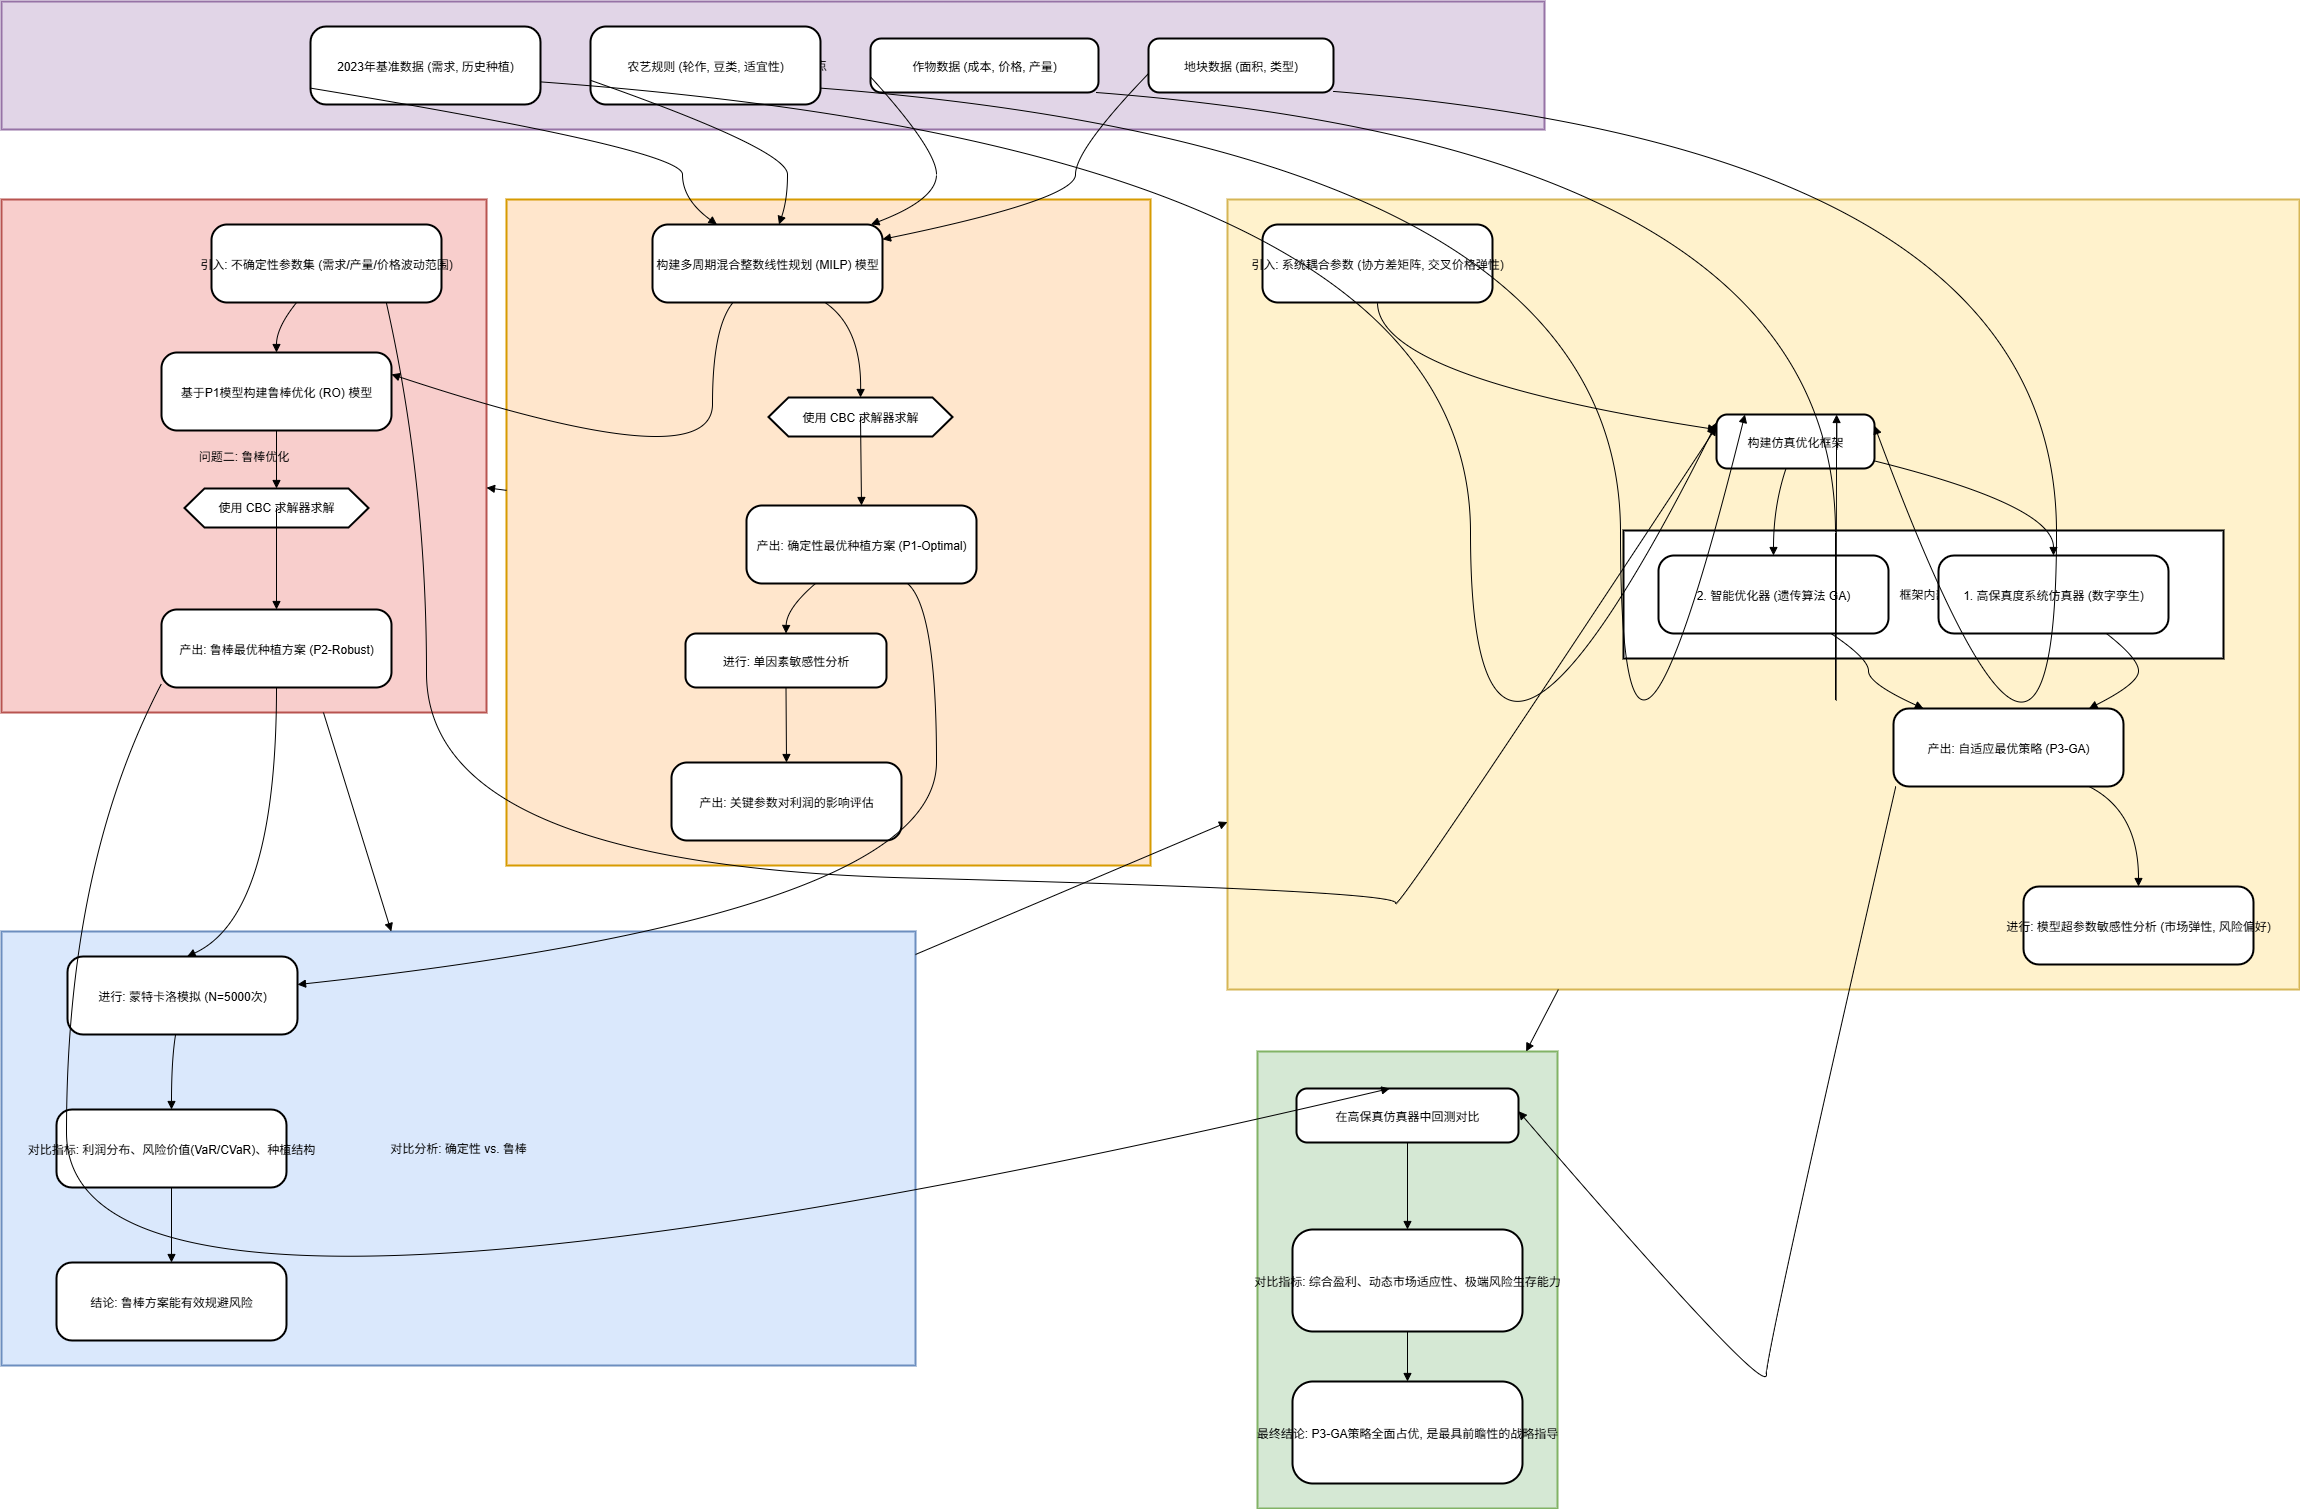
\includegraphics[width=0.7\textwidth]{../figures/all.png}
	\caption{整体框架}
	\label{fig:all}
\end{figure}


\section{模型假设}

\begin{enumerate}
	\item 假设2023年的农作物产量恰好满足当期市场需求,该年的产销数据可作为后续模型中市场预期销售量的基准。
	\item 假设附件所提供的全部数据均真实、准确,可作为模型的基础输入。
	\item 假设该乡村在农产品市场中为价格接受者,其任何一种作物的产量变化均不足以影响该作物的市场结算价格。
	\item 假设所有在预期内或可降价出售的农产品均能当季顺利售出,模型不考虑仓储、物流运输、市场交易以及产品损耗等环节产生的额外成本或收益影响。
\end{enumerate}


\section{符号说明}

\begin{table}[H]
	\centering
	\caption{符号说明}
	\begin{tabular}{ll}
		\toprule
		符号                 & 说明                                \\
		\midrule

		$i, I$             & 地块的索引与集合                          \\
		$j, J$             & 作物的索引与集合                          \\
		$k, K$             & 季节的索引与集合                          \\
		$y, Y$             & 年份的索引与集合(2024-2030)               \\
		$J_{\text{bean}}$  & 所有豆类作物的集合                         \\

		$A_i$              & 地块$i$ 的可用面积                       \\
		$C_j$              & 作物$j$ 的单位面积种植成本                   \\
		$P_j$              & 作物$j$ 的单位重量销售价格                   \\
		$\text{Yield}_j$   & 作物$j$ 的单位面积产量                     \\
		$\text{Demand}_j$  & 作物$j$ 的每季预期市场销售量                  \\
		$\text{Past}_{ij}$ & 地块$i$ 在2023年是否种植了作物 $j$ 的0-1参数    \\
		$S_{ijk}$          & 地块$i$ 在季节 $k$ 是否适宜种植作物 $j$ 的0-1参数 \\
		$A_{\min}$         & 单个地块上允许种植某种作物的最小面积阈值              \\
		$N_j$              & 作物$j$ 在单季内允许种植的最大分散地块数量           \\
		$M$                & 大M方法中的一个足够大的正数                    \\
		\bottomrule
	\end{tabular}
\end{table}

\section{数据分析与预处理}

在构建优化模型之前,对基础数据进行系统性的分析与处理是确保模型有效性的前提。本章旨在对该乡村的耕地结构、农作物种植现状及关键经济参数进行定量剖析,为后续模型提供必需参数,并洞察该农业系统的内在结构与潜在的经济驱动力。

\subsection{耕地资源与农学含义分析}

农业生产的边界首先由其拥有的土地资源所决定。该乡村的耕地由露天耕地与设施大棚两部分构成。如图\ref{fig:land_structure}所示,露天耕地总面积为1201亩,主要类型为梯田(52\%)与平旱地(30\%)。这种以旱作为主的土地结构,从农学角度揭示了该地区可能面临水资源约束和土壤保持的挑战,使得耐旱作物的选择和水土保持措施显得尤为重要。设施农业方面,16个普通大棚和4个智慧大棚共提供了12亩受控环境的耕作面积,为高附加值作物的生产提供了可能。这一系列的土地类型、面积及适种信息,将直接转化为优化模型中的地块面积参数$A_i$与种植适宜性参数$S_{ijk}$。

\begin{figure}[t]
	\centering
	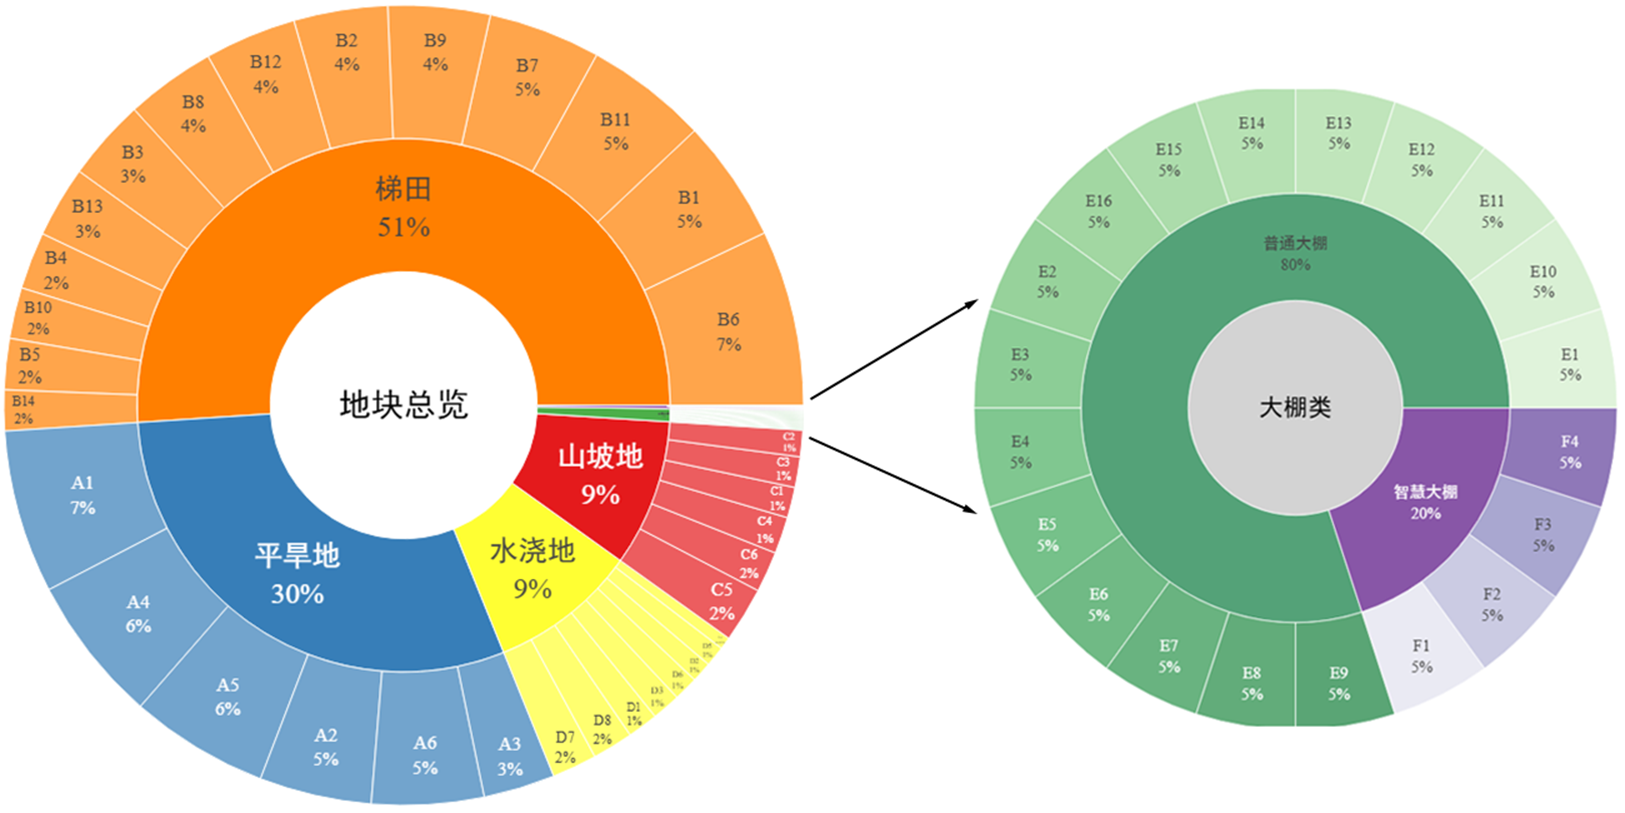
\includegraphics[width=0.8\textwidth]{../figures/0_1.png}
	\caption{露天耕地结构(左)与大棚耕地结构(右)分布图}
	\label{fig:land_structure}
\end{figure}

\subsection{农作物种植现状与经济效益分析}

为建立后续模型的经济基准,我们对2023年的农作物生产数据进行分析。图\ref{fig:production_rank}依据总产量对2023年种植的各类作物进行排序,揭示了当前农业生产的整体格局。小麦、玉米等粮食作物在总产量上占据绝对主导地位,是维系该乡村农业经济的“压舱石”。根据模型假设,2023年的各类作物产量被视为恰好满足市场需求的水平,因此这一产量数据为模型中的基准市场需求参数$Demand_j$的设定提供了直接依据。

\begin{figure}[h]
	\centering
	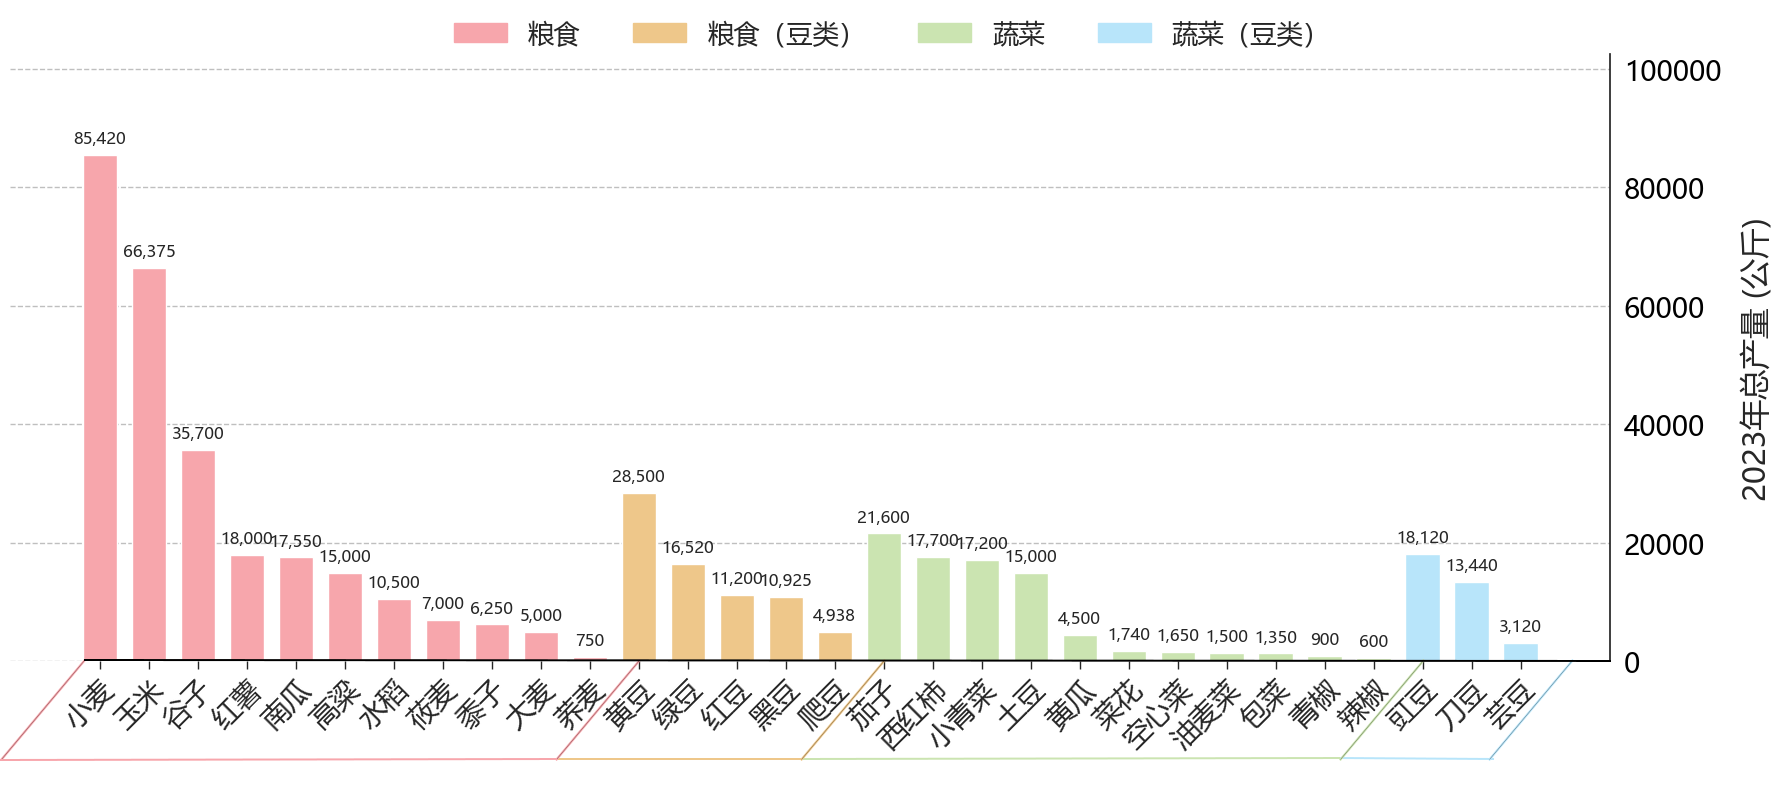
\includegraphics[width=0.9\textwidth]{../figures/0_2.png}
	\caption{2023年各类农作物总产量排名}
	\label{fig:production_rank}
\end{figure}


经济效益是驱动种植决策的核心。我们结合附件数据核算了各类作物的亩均净利润(见图\ref{fig:profit_per_mu})。分析发现,作物间的盈利能力存在巨大差异。羊肚菌、大白菜等经济作物展现出极高的亩均利润,而粮食作物的单位利润则偏低。这种显著的利润分化揭示了该乡村面临的经典经济学权衡:高利润经济作物如同高风险高回报的“成长股”,而粮食作物则像是收益稳定、保障基本盘的“债券”。因此,最优种植策略的本质,可以类比为在现代投资组合理论的指导下,构建一个平衡风险与收益的、最优化的“农业资产包”。

\begin{figure}[htbp]
	\centering
	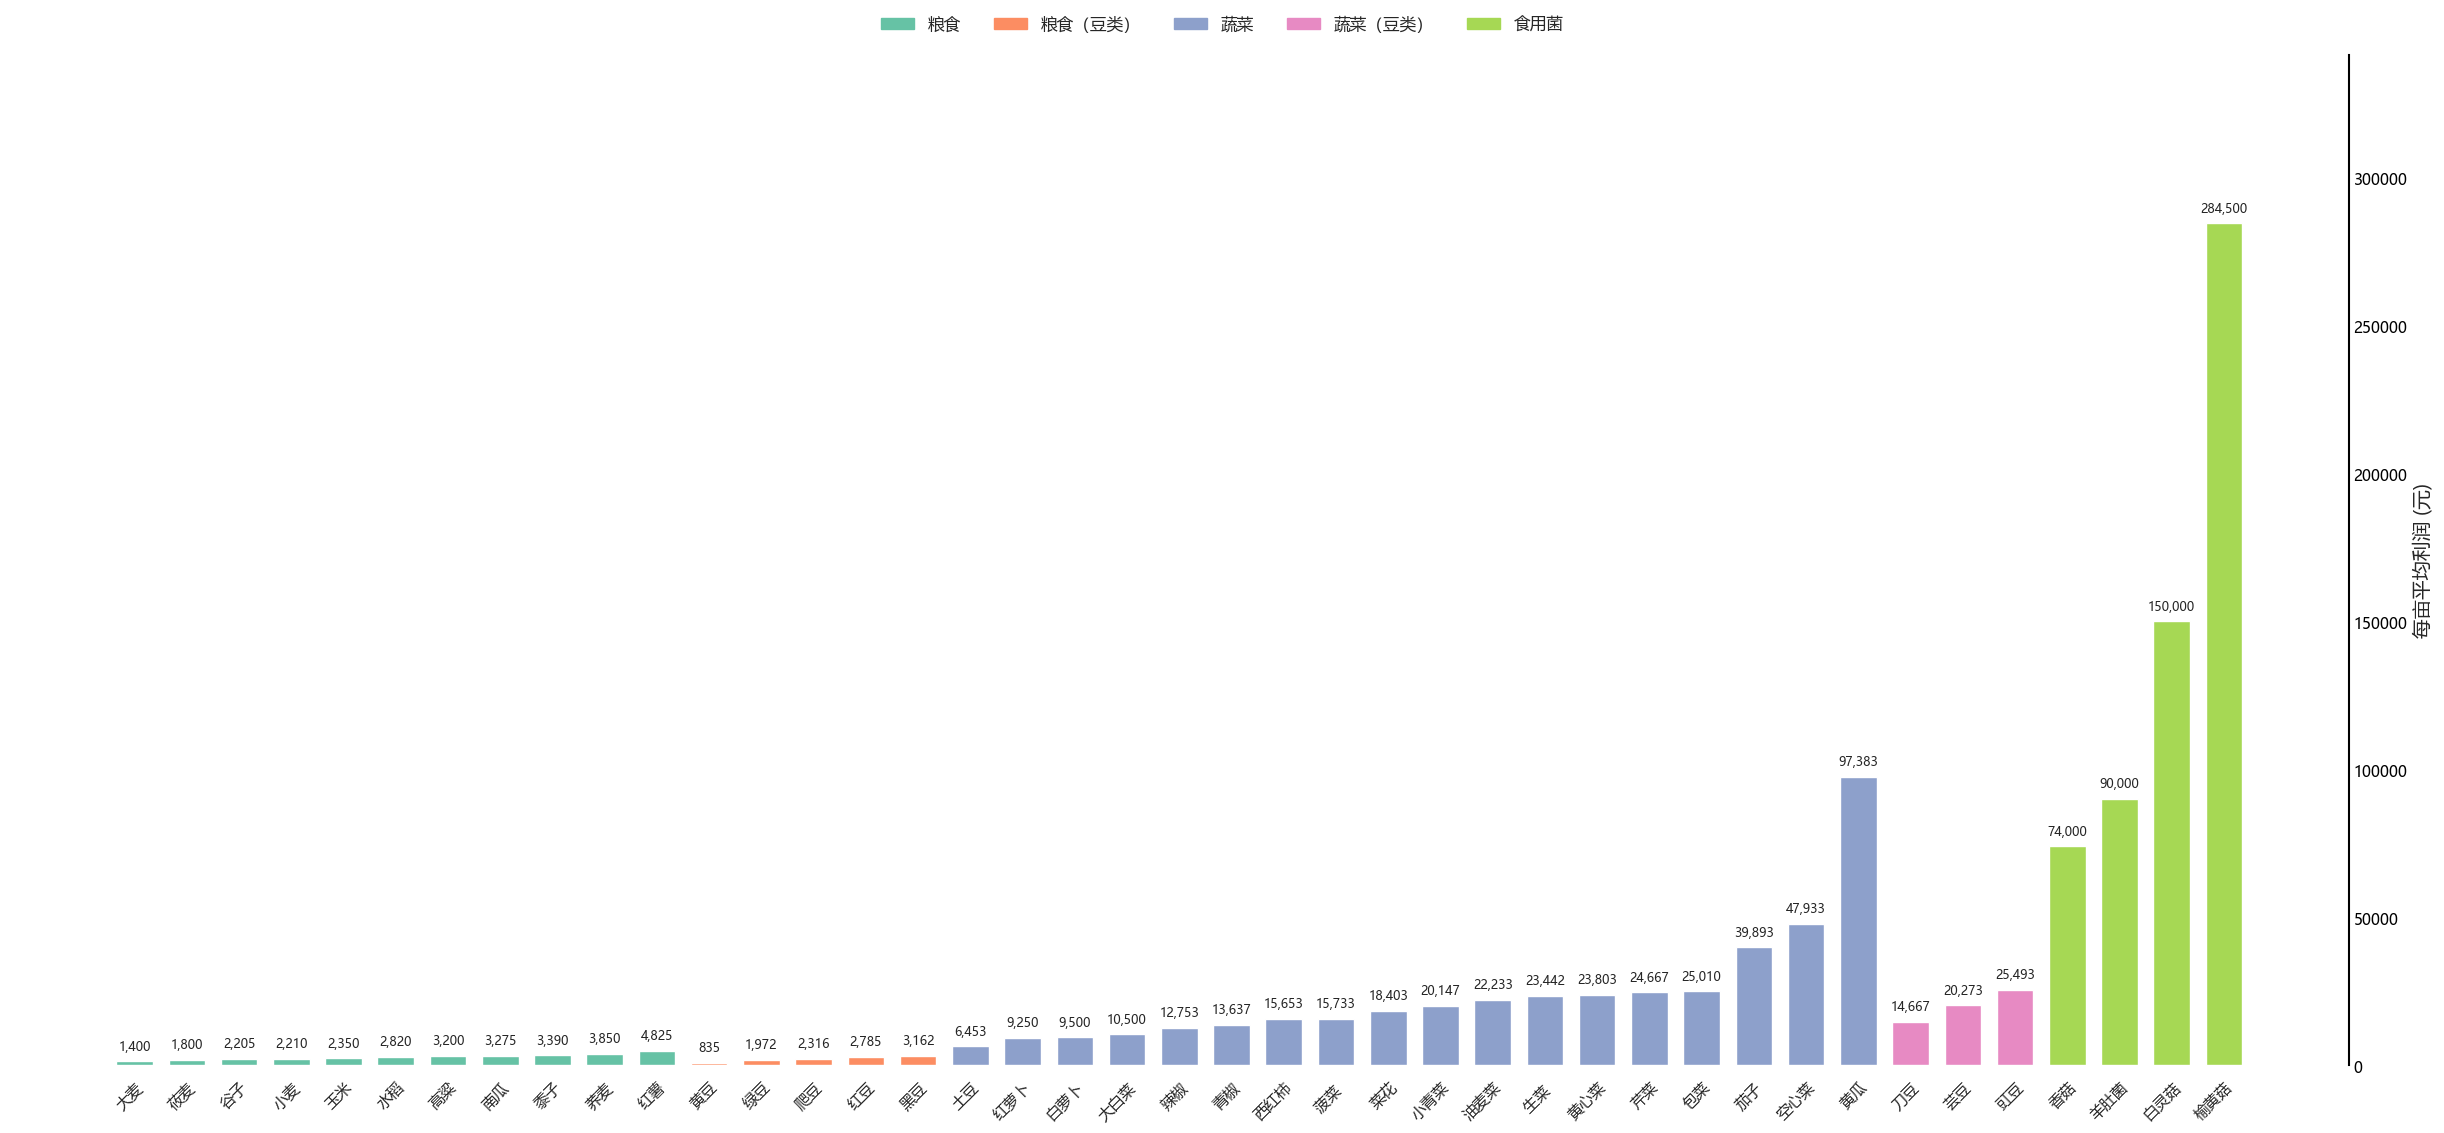
\includegraphics[width=0.9\textwidth]{../figures/0_3.png}
	\caption{各类农作物亩均净利润对比分析}
	\label{fig:profit_per_mu}
\end{figure}

\section{问题一:确定性环境下的多周期优化模型}

问题一旨在为该乡村规划2024年至2030年共七年的农作物种植策略。该问题本质上是一个在完全信息假设下的多周期资源分配问题。从微观经济学视角看,这相当于将该乡村抽象为一个理性的经济主体,其在拥有固定的生产技术、资源禀赋和已知的市场参数条件下,追求长期利润的最大化。由于决策变量中既包含连续的种植面积,也包含是否种植的离散选择,该问题能够被精确地构建为一个大规模的多周期混合整数线性规划(MILP)模型。本章将详细阐述该模型的构建、求解与分析过程,旨在为后续更复杂的分析提供一个确定性环境下的最优基准。

模型的顶层设计如图\ref{fig:milp_framework}所示,它清晰地展示了模型的输入、处理核心与输出。该框架整合了土地资源、作物属性、经济参数和农艺规则,通过MILP求解器进行优化,最终生成最优的七年种植方案与相应的经济效益预测。

% \begin{figure}[htbp]
%     \centering
%     \includegraphics[width=0.8\textwidth]{figures/milp_framework.png}
%     \caption{问题一的混合整数线性规划模型概念框架图。该框架整合了多源输入数据,通过优化核心生成最优种植方案与经济预测,为确定性环境下的决策提供了系统性方法。}
%     \label{fig:milp_framework}
% \end{figure}

\subsection{模型构建}


为将该乡村的长期种植规划问题转化为一个可求解的数学模型,我们构建了一个多周期混合整数线性规划(MILP)模型。该模型以古典微观经济学中的厂商理论为基础,将乡村视为一个追求长期利润最大化的理性决策主体。模型的构建过程遵循模块化原则,依次定义了决策变量、目标函数和约束条件三个核心部分。

\subsubsection{决策变量}

模型的决策核心在于如何在给定的时间和空间维度上分配种植资源。为此,我们定义了以下三组核心决策变量,它们共同构成了完整的七年种植方案:
\begin{itemize}
	\item \textbf{种植面积变量 ($x_{ijky}$)}: 这是一个连续变量,代表在年份 $y \in Y$ 的季节 $k \in K$,于地块 $i \in I$ 安排种植作物 $j \in J$ 的具体面积。该变量是模型的核心,直接关联到成本与产出。
	\item \textbf{种植决策变量 ($u_{ijky}$)}: 这是一个二进制变量,用于表征种植行为的有无。当且仅当在地块 $i$ 的 $y$ 年 $k$ 季实际安排了作物 $j$ 的种植(即 $x_{ijky} > 0$)时,$u_{ijky}$ 取值为1,否则为0。该变量主要用于处理与规模化经营相关的逻辑约束。
	\item \textbf{年度种植状态变量 ($z_{ijy}$)}: 这是一个年度层面的二进制变量。若在年份 $y$ 的任何一个季节,地块 $i$ 安排了作物 $j$ 的种植,则 $z_{ijy}$ 取值为1,否则为0。该变量用于聚合季节性种植信息,以简化跨年度农艺约束的表达。
\end{itemize}
此外,为处理产出与销售环节的逻辑,引入了两组关键的辅助变量:
\begin{itemize}
	\item \textbf{正常销售量 ($Sales_{jky}$)}: 表示作物 $j$ 在年份 $y$ 季节 $k$ 的总产量中,在预期市场需求内,按正常市场价格销售的数量。
	\item \textbf{超产销售量 ($OverSales_{jky}$)}: 表示作物 $j$ 在年份 $y$ 季节 $k$ 的总产量中,超出预期市场需求后,进行降价处理的销售数量。
\end{itemize}

\subsubsection{目标函数}

模型的目标是最大化在整个七年规划期(2024-2030)内的累计净利润。根据题目设定的两种不同市场情景,分别构建对应的目标函数。

\textbf{情景一:超产滞销}

在此情景下,任何超出市场预期需求量的产量均无法转化为经济收益,其价值为零。因此,总收益仅由正常销售部分贡献。目标函数定义为:
\begin{equation}
	\max \sum_{y \in Y} \sum_{k \in K} \left( \sum_{j \in J} P_j \cdot Sales_{jky} - \sum_{j \in J} \sum_{i \in I} C_j \cdot x_{ijky} \right)
\end{equation}
其中,$P_j$ 代表作物 $j$ 的单位重量销售价格,$C_j$ 代表作物 $j$ 的单位面积种植成本。

\textbf{情景二:超产降价出售}

在此情景下,超产部分仍能以正常销售价格的50\%售出,为乡村带来额外收益。这使得目标函数中包含了超产销售所贡献的价值。目标函数更新为:
\begin{equation}
	\max \sum_{y \in Y} \sum_{k \in K} \left( \sum_{j \in J} (P_j \cdot Sales_{jky} + 0.5 \cdot P_j \cdot OverSales_{jky}) - \sum_{j \in J} \sum_{i \in I} C_j \cdot x_{ijky} \right)
\end{equation}
该目标函数更全面地反映了具有一定市场弹性时的经济状况。

\subsubsection{约束条件}

为了确保模型生成的种植方案在现实中是可行的、在农艺上是科学的,并且在生态上是可持续的,我们构建了一个严密的约束体系。该体系将农业生产的各个环节,从土地资源的物理限制到市场销售的经济规则,再到长期的生态维护要求,均纳入了数学模型的考量范围之内。

\textbf{1. 总产量约束}

该约束是连接农业生产与市场流通的核心纽带,它确保了特定作物在某个时期的总产量等于其正常销售量与超产销售量之和。

\begin{equation}
	Yield_j \cdot \sum_{i \in I} x_{ijky} = Sales_{jky} + OverSales_{jky} \quad \forall j \in J, k \in K, y \in Y
\end{equation}
其中,$Yield_j$ 是作物 $j$ 的单位面积产量。对于情景一,只需令 $OverSales_{jky}$ 恒等于0即可。

\textbf{2. 市场销售约束}

此约束为每种作物的正常价格销售量设置了天花板,它反映了市场在正常价格下的有限吸纳能力,是模型进行生产规模决策时的重要经济信号。

\begin{equation}
	Sales_{jky} \le Demand_j \quad \forall j \in J, k \in K, y \in Y
\end{equation}
其中,$Demand_j$ 是作物 $j$ 的每季预期市场销售量上限。此约束为每种作物的正常价格销售量设置了天花板,它反映了市场在正常价格下的有限吸纳能力,是模型进行生产规模决策时的重要经济信号。

\textbf{3. 土地面积约束}

这是一个基础的物理资源约束,它规定在任意地块上,于特定时期种植的所有作物的总面积之和,不能超过该地块的实际可用总面积。

\begin{equation}
	\sum_{j \in J} x_{ijky} \le A_i \quad \forall i \in I, k \in K, y \in Y
\end{equation}
其中,$A_i$ 是地块 $i$ 的可用面积。

\textbf{4. 种植适宜性约束}

此约束通过预设的农学参数,将因地制宜的科学种植原则制度化,强制任何种植活动只能发生在适宜的土地类型和季节条件下。

\begin{equation}
	x_{ijky} \le S_{ijk} \cdot M \quad \forall i \in I, j \in J, k \in K, y \in Y
\end{equation}
其中,$S_{ijk}$ 是一个二进制参数,当作物 $j$ 适宜在地块 $i$ 的季节 $k$ 种植时为1,否则为0;$M$ 是一个足够大的正数。

\textbf{5. 规模化经营约束}

这组约束旨在将田间管理的经济学原理量化。它通过逻辑变量 $u_{ijky}$ 将种植决策与种植面积相绑定,确保了种植行为的规模化,避免了因种植活动过于零散而导致的管理成本飙升和生产效率下降。

\begin{align}
	 & x_{ijky} \le A_i \cdot u_{ijky} \quad \forall i, j, k, y      \\
	 & x_{ijky} \ge A_{\min} \cdot u_{ijky} \quad \forall i, j, k, y \\
	 & \sum_{i \in I} u_{ijky} \le N_j \quad \forall j, k, y
\end{align}
其中,$A_{\min}$ 是单个地块上允许种植某种作物的最小面积阈值,$N_j$ 是作物 $j$ 在单季内允许种植的最大分散地块数量。

\textbf{6. 忌重茬约束}

该约束是保障土地可持续利用和维持长期生产力的关键农艺要求。它通过年度状态变量 $z_{ijy}$,严格禁止任何同种作物在同一地块上连续两年种植。该约束通过2023年的历史数据与未来年份衔接,实现了跨越整个规划期的轮作要求,是防止土壤病虫害累积和肥力退化的核心生态约束。

\begin{align}
	 & z_{ijy} \ge u_{ijky} \quad \forall i, j, k, y                                       \\
	 & z_{ij,2024} + Past_{ij} \le 1 \quad \forall i, j                                    \\
	 & z_{ijy} + z_{ij,y+1} \le 1 \quad \forall i, j, \text{ and } y \in \{2024,...,2029\}
\end{align}
其中,$Past_{ij}$ 是一个历史数据参数,若地块 $i$ 在2023年种植了作物 $j$ 则为1,否则为0。

\textbf{7. 豆类种植比例以及田间管理便利性等多重约束条件的影响}

此约束旨在通过强制性的豆科作物轮作来改良土壤结构和提升土壤肥力,是一项重要的生态农艺措施。豆科作物的根瘤菌固氮作用是实现农业系统内部氮循环、减少对外部化肥依赖的关键。模型采用一个为期三年的滑动窗口,要求每个地块在任何连续三年内,必须至少安排一次豆科作物的种植,从而将可持续发展的理念内生化到优化模型中。

\begin{align}
	 & \sum_{j \in J_{\text{bean}}} (Past_{ij} + z_{ij,2024} + z_{ij,2025}) \ge 1 \quad \forall i                                   \\
	 & \sum_{j \in J_{\text{bean}}} (z_{ijy} + z_{ij,y+1} + z_{ij,y+2}) \ge 1 \quad \forall i, \text{ and } y \in \{2024,...,2028\}
\end{align}
其中,$J_{\text{bean}}$ 是所有豆类作物的集合。

\subsubsection{优化模型的整合呈现}

综上所述,将问题一中的两种不同市场情景分别构建为独立的多周期混合整数线性规划(MILP)模型。每个模型共享相同的决策变量定义和大部分农艺及管理约束,但在目标函数和产量-销售衔接约束上有所区别。下面分别呈现这两个模型的完整数学范式。

\subsubsection{模型一:超产部分滞销浪费情景}
在此情景下,任何超出市场预期需求量的产量均无法产生经济价值。模型的优化目标是最大化由正常销售部分贡献的利润。其完整的数学形式如下:
\begin{align}
\max \quad & \sum_{y \in Y} \sum_{k \in K} \left( \sum_{j \in J} P_j \cdot Sales_{jky} - \sum_{j \in J} \sum_{i \in I} C_j \cdot x_{ijky} \right) \\
\text{s.t.} \quad & \left\{
    \begin{array}{l}
        \text{Yield}_j \cdot \sum_{i \in I} x_{ijky} \ge Sales_{jky} \quad \forall j,k,y                                  \\
        Sales_{jky} \le \text{Demand}_j \quad \forall j,k,y                                                          \\
        \sum_{j \in J} x_{ijky} \le A_i \quad \forall i,k,y                                                          \\
        A_{\min} \cdot u_{ijky} \le x_{ijky} \le A_i \cdot u_{ijky} \cdot S_{ijk} \quad \forall i,j,k,y                \\
        \sum_{i \in I} u_{ijky} \le N_j \quad \forall j,k,y                                                          \\
        z_{ijy} \ge u_{ijky} \quad \forall i,j,k,y                                                                   \\
        z_{ij,2024} + \text{Past}_{ij} \le 1 \quad \forall i,j                                                       \\
        z_{ijy} + z_{ij,y+1} \le 1 \quad \forall i,j, \; y \in \{2024,...,2029\}                                      \\
        \sum_{j \in J_{bean}} (\text{Past}_{ij} + z_{ij,2024} + z_{ij,2025}) \ge 1 \quad \forall i                     \\
        \sum_{j \in J_{bean}} (z_{ijy} + z_{ij,y+1} + z_{ij,y+2}) \ge 1 \quad \forall i, \; y \in \{2024,...,2028\}    \\
        x_{ijky}, Sales_{jky} \ge 0 \quad \forall i,j,k,y                                                            \\
        u_{ijky}, z_{ijy} \in \{0, 1\} \quad \forall i,j,k,y
    \end{array}
    \right.
\end{align}

\subsubsection{模型二:超产部分降价出售情景}
在此情景下,超出市场预期的产量仍能以基准价格的50\%售出,为乡村带来额外收益。模型的目标函数和产量约束相应调整,以反映这一变化。其完整的数学形式如下:
\begin{align}
\max \quad & \sum_{y \in Y} \sum_{k \in K} \left( \sum_{j \in J} (P_j \cdot Sales_{jky} + 0.5 \cdot P_j \cdot \text{OverSales}_{jky}) - \sum_{j \in J} \sum_{i \in I} C_j \cdot x_{ijky} \right) \\
\text{s.t.} \quad & \left\{
    \begin{array}{l}
        \text{Yield}_j \cdot \sum_{i \in I} x_{ijky} = Sales_{jky} + \text{OverSales}_{jky} \quad \forall j,k,y        \\
        Sales_{jky} \le \text{Demand}_j \quad \forall j,k,y                                                          \\
        \sum_{j \in J} x_{ijky} \le A_i \quad \forall i,k,y                                                          \\
        A_{\min} \cdot u_{ijky} \le x_{ijky} \le A_i \cdot u_{ijky} \cdot S_{ijk} \quad \forall i,j,k,y                \\
        \sum_{i \in I} u_{ijky} \le N_j \quad \forall j,k,y                                                          \\
        z_{ijy} \ge u_{ijky} \quad \forall i,j,k,y                                                                   \\
        z_{ij,2024} + \text{Past}_{ij} \le 1 \quad \forall i,j                                                       \\
        z_{ijy} + z_{ij,y+1} \le 1 \quad \forall i,j, \; y \in \{2024,...,2029\}                                      \\
        \sum_{j \in J_{bean}} (\text{Past}_{ij} + z_{ij,2024} + z_{ij,2025}) \ge 1 \quad \forall i                     \\
        \sum_{j \in J_{bean}} (z_{ijy} + z_{ij,y+1} + z_{ij,y+2}) \ge 1 \quad \forall i, \; y \in \{2024,...,2028\}    \\
        x_{ijky}, Sales_{jky}, \text{OverSales}_{jky} \ge 0 \quad \forall i,j,k,y                                     \\
        u_{ijky}, z_{ijy} \in \{0, 1\} \quad \forall i,j,k,y
    \end{array}
    \right.
\end{align}

\subsection{模型求解与结果分析}

\subsubsection{模型求解}

本研究构建的优化模型属于大规模多周期混合整数线性规划(MILP)问题,其特点是包含大量连续变量(如种植面积$x_{ijky}$)与二进制变量(如种植决策$u_{ijky}$和$z_{ijy}$),且约束条件复杂。针对此类问题,必须采用能够有效处理整数约束的专用求解器。综合考虑求解性能、算法可靠性与研究的可复现性,我们选择采用开源求解器COIN-OR Branch and Cut(CBC)进行模型求解。

选择CBC求解器的核心原因在于其算法的适用性与强大功能。CBC求解器是基于成熟的“分支与切割”(Branch and Cut)算法构建的,这是一种专门用于求解混合整数规划问题的精确算法。对于本模型而言,“分支”过程能够系统性地探索由“是否种植”等离散决策变量($u_{ijky}$和$z_{ijy}$)构成的庞大组合空间;而“切割”过程则通过在求解过程中动态添加割平面约束,有效收紧线性松弛问题的可行域,从而大幅提升寻找最优整数解的效率。更重要的是,作为一种精确算法,CBC能够在给予足够计算时间的情况下,保证找到问题的全局最优解,并提供最优性证明。这确保了我们最终获得的七年种植策略在模型框架下是数学意义上的最佳方案,而非局部最优或近似解。此外,CBC作为COIN-OR(COmputational INfrastructure for Operations Research)项目的一部分,其开源属性不仅消除了商业软件的许可成本,更提升了研究的透明度与可复现性,便于其他研究者验证和拓展我们的工作。我们将借助Python中的Pyomo建模语言构建数学模型,并调用CBC求解器完成计算。

\subsubsection{总体经济效益与市场情景对比}

% 模型的求解结果揭示了市场销售渠道对总体经济效益的决定性影响。如图\ref{fig:profit_comparison}所示,在超产部分完全滞销的情景下,模型预测的七年累计总利润为4120万元。然而,若允许超产部分以五折价格进行销售,最优总利润则能显著提升至5860万元,增幅高达42.2\%。这一结果定量地证明了拓展农产品销售渠道、增强市场消化能力的巨大经济价值,为乡村制定产业政策提供了明确的方向。

模型的求解结果揭示了市场销售渠道对总体经济效益的决定性影响。在超产部分完全滞销的情景下,模型预测的七年累计总利润为4120万元。然而,若允许超产部分以五折价格进行销售,最优总利润则能显著提升至5860万元,增幅高达42.2\%。这一结果定量地证明了拓展农产品销售渠道、增强市场消化能力的巨大经济价值,为乡村制定产业政策提供了明确的方向。

% \begin{figure}[htbp]
%     \centering
%     \includegraphics[width=0.7\textwidth]{figures/profit_comparison.png}
%     \caption{两种市场情景下的最优七年累计总利润对比。结果表明,允许超产部分降价销售能够极大地提升该乡村的总体经济效益。}
%     \label{fig:profit_comparison}
% \end{figure}

\subsubsection{最优种植结构的时间演化}

最优种植策略并非静态的重复,而是在时间维度上呈现出动态的轮作模式。图\ref{fig:portfolio_evolution}展示了在情景二下,三大类作物(粮食作物、经济作物、食用菌)总种植面积在七年规划期内的演化趋势。可以观察到,高附加值的经济作物和食用菌始终占据了大部分的种植面积,是利润的主要来源。同时,各类作物的种植面积呈现周期性波动,这正是模型为了满足忌重茬和豆类轮作等农艺约束而进行的自主调整,形成了一个可持续的、动态平衡的种植系统。

\begin{figure}[htbp]
    \centering
    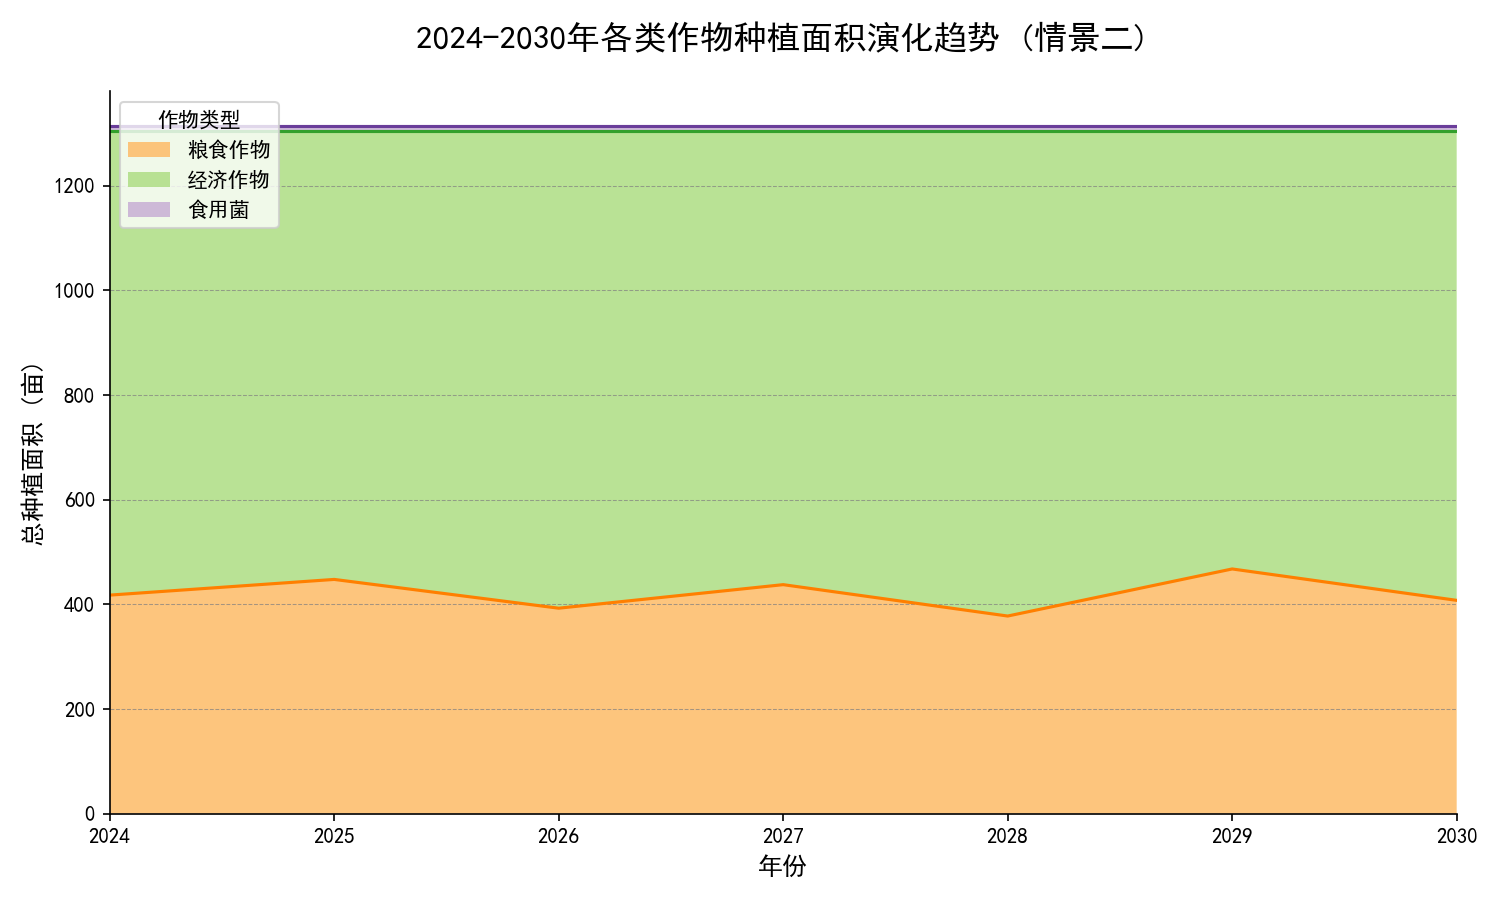
\includegraphics[width=0.95\textwidth]{figs/3问题一/portfolio_evolution.png}
    \caption{最优种植方案下三大类作物总种植面积的七年动态演化图(情景二)。该图揭示了模型在追求利润最大化的同时,为满足农艺约束而形成的动态轮作模式。}
    \label{fig:portfolio_evolution}
\end{figure}

\subsubsection{土地资源利用的空间分布格局}

除了时间维度的动态性,最优方案在空间上也表现出精细化的资源配置策略。图\ref{fig:land_utilization}通过热力图的形式,展示了部分代表性地块在七年间的作物类型分配情况。图中可以清晰地看到,水浇地和智慧大棚等高质量土地资源被优先用于种植高利润的两季蔬菜和食用菌,实现了“好钢用在刀刃上”。而平旱地和梯田则主要承担了粮食作物和豆类的轮作任务。这种空间上的差异化布局,是模型根据不同地块的生产效率和适宜性进行优化配置的直观体现。

\begin{figure}[htbp]
    \centering
    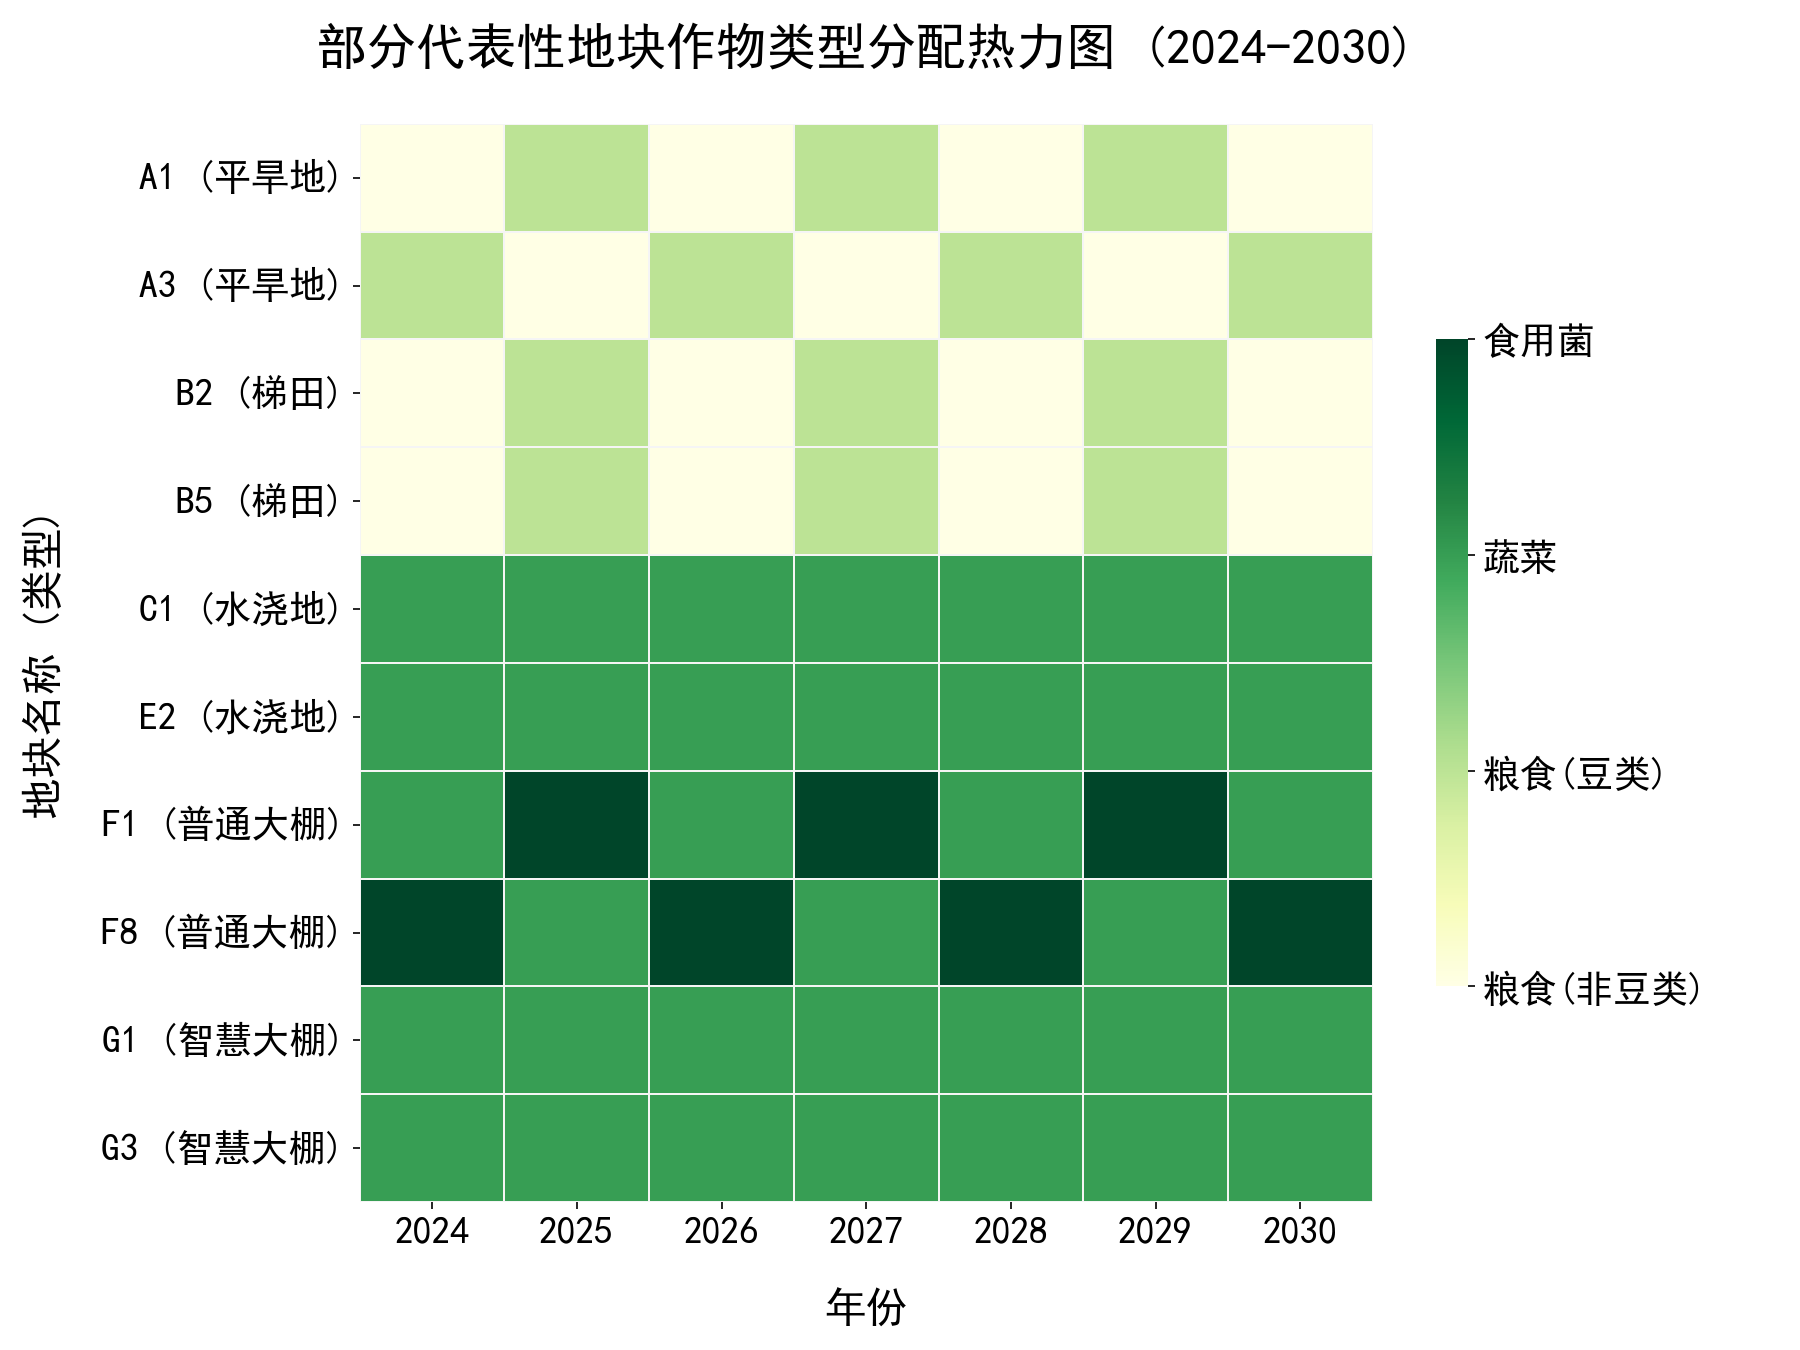
\includegraphics[width=0.95\textwidth]{figs/3问题一/land_utilization.png}

    \caption{部分代表性地块在七年规划期内的作物类型分配热力图。不同颜色代表不同作物类型,展示了模型对不同质量土地资源的差异化、精细化利用策略。}
    \label{fig:land_utilization}
\end{figure}

\subsubsection{影子价格分析}

为了探究限制乡村发展的关键瓶颈,我们对模型中的资源约束进行了影子价格分析。影子价格(Shadow Price)在经济学上代表着当某种资源增加一个单位时,所能带来的最优目标函数的增量,是衡量资源稀缺性和经济价值的有效指标。如图\ref{fig:shadow_price}所示,智慧大棚和水浇地的影子价格远高于其他类型的土地资源。这表明,高效率的设施农业用地和优质的水源保障是当前制约该乡村农业总产值提升的最关键因素。这一结论为未来的投资方向提供了有力的决策依据:增加对智慧大棚建设和水利设施改善的投入,将是撬动整个乡村经济增长的最有效杠杆。

\begin{figure}[htbp]
    \centering
    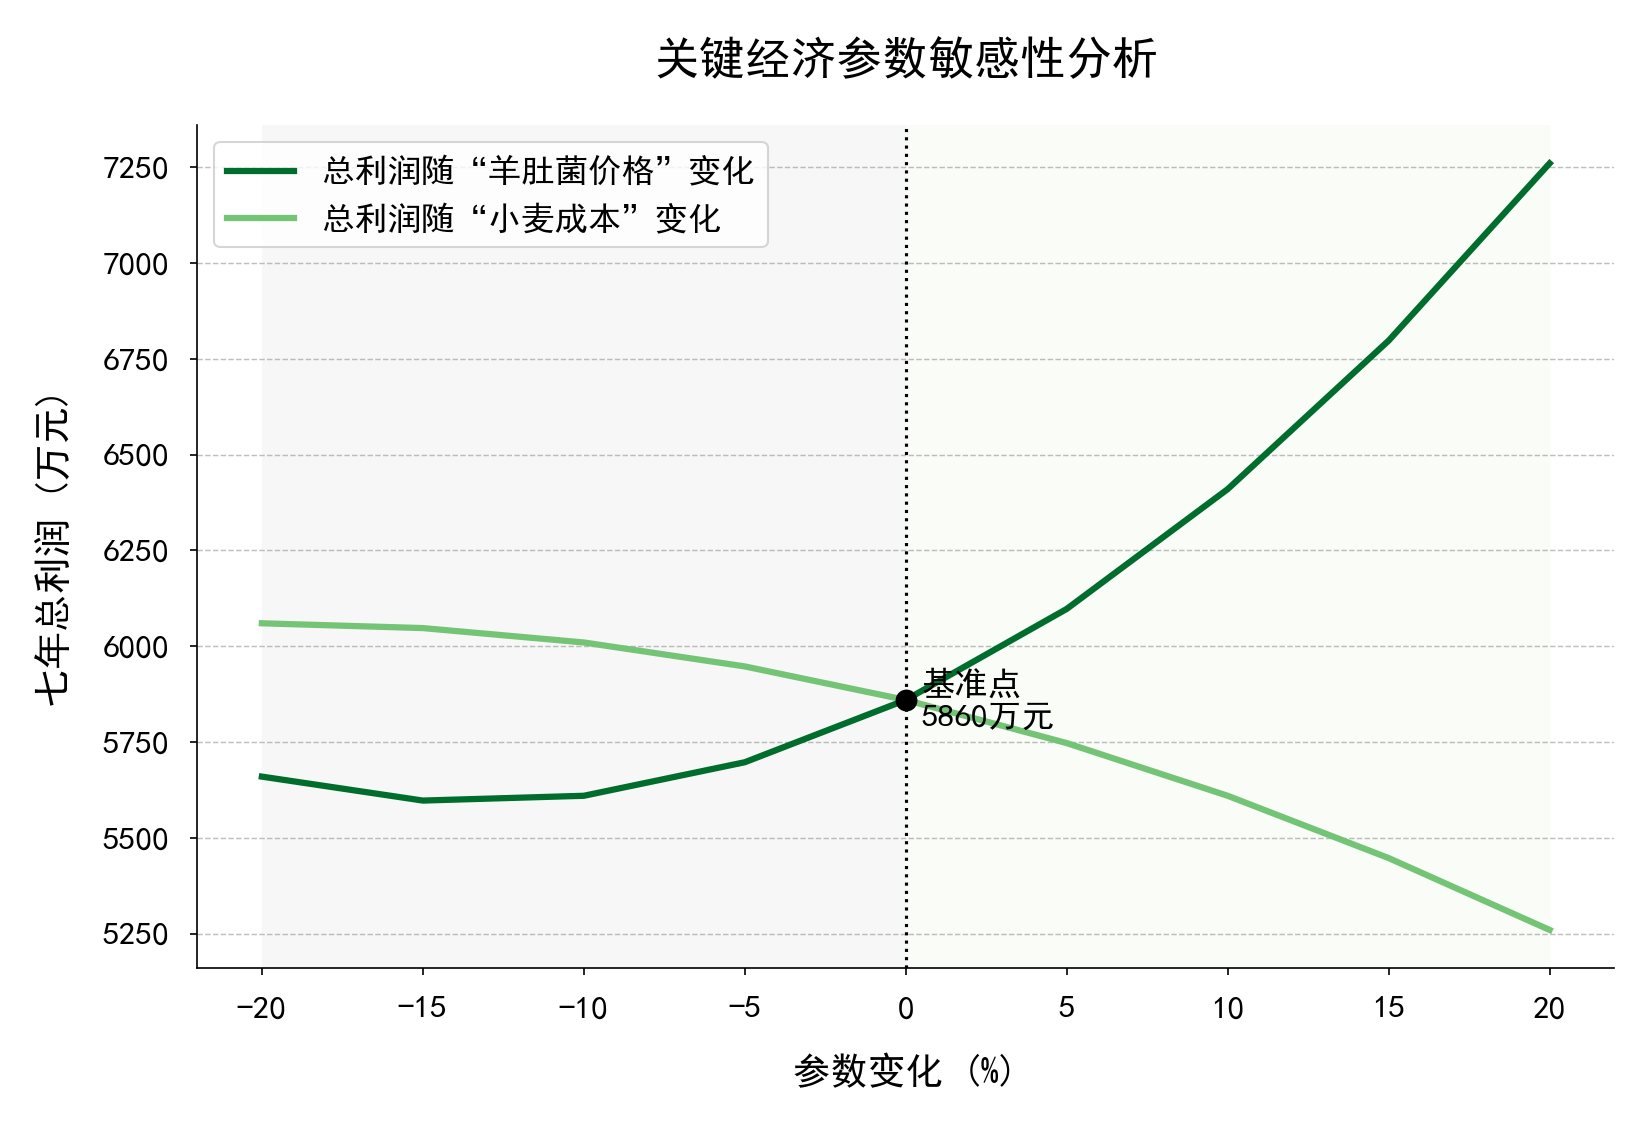
\includegraphics[width=0.8\textwidth]{figures/shadow_price.png}
    \caption{主要土地资源约束的影子价格分析。结果量化了不同类型土地资源的边际经济价值,揭示了智慧大棚和水浇地是当前最具价值的稀缺资源。}
    \label{fig:shadow_price}
\end{figure}

\subsubsection{敏感性分析}

最后,我们通过敏感性分析来评估确定性最优解在面对外部参数扰动时的稳定性。图\ref{fig:price_sensitivity}展示了总利润对高价值经济作物(以羊肚菌为例)销售价格和主要粮食作物(以小麦为例)种植成本的敏感性。结果显示,总利润对羊肚菌价格的弹性极高,其价格的微小波动便能引起总利润的剧烈变化。这揭示了当前利润最大化方案的脆弱性:它高度依赖于少数几种高价值作物的市场表现,构成了主要的市场风险来源。

\begin{figure}[htbp]
    \centering
    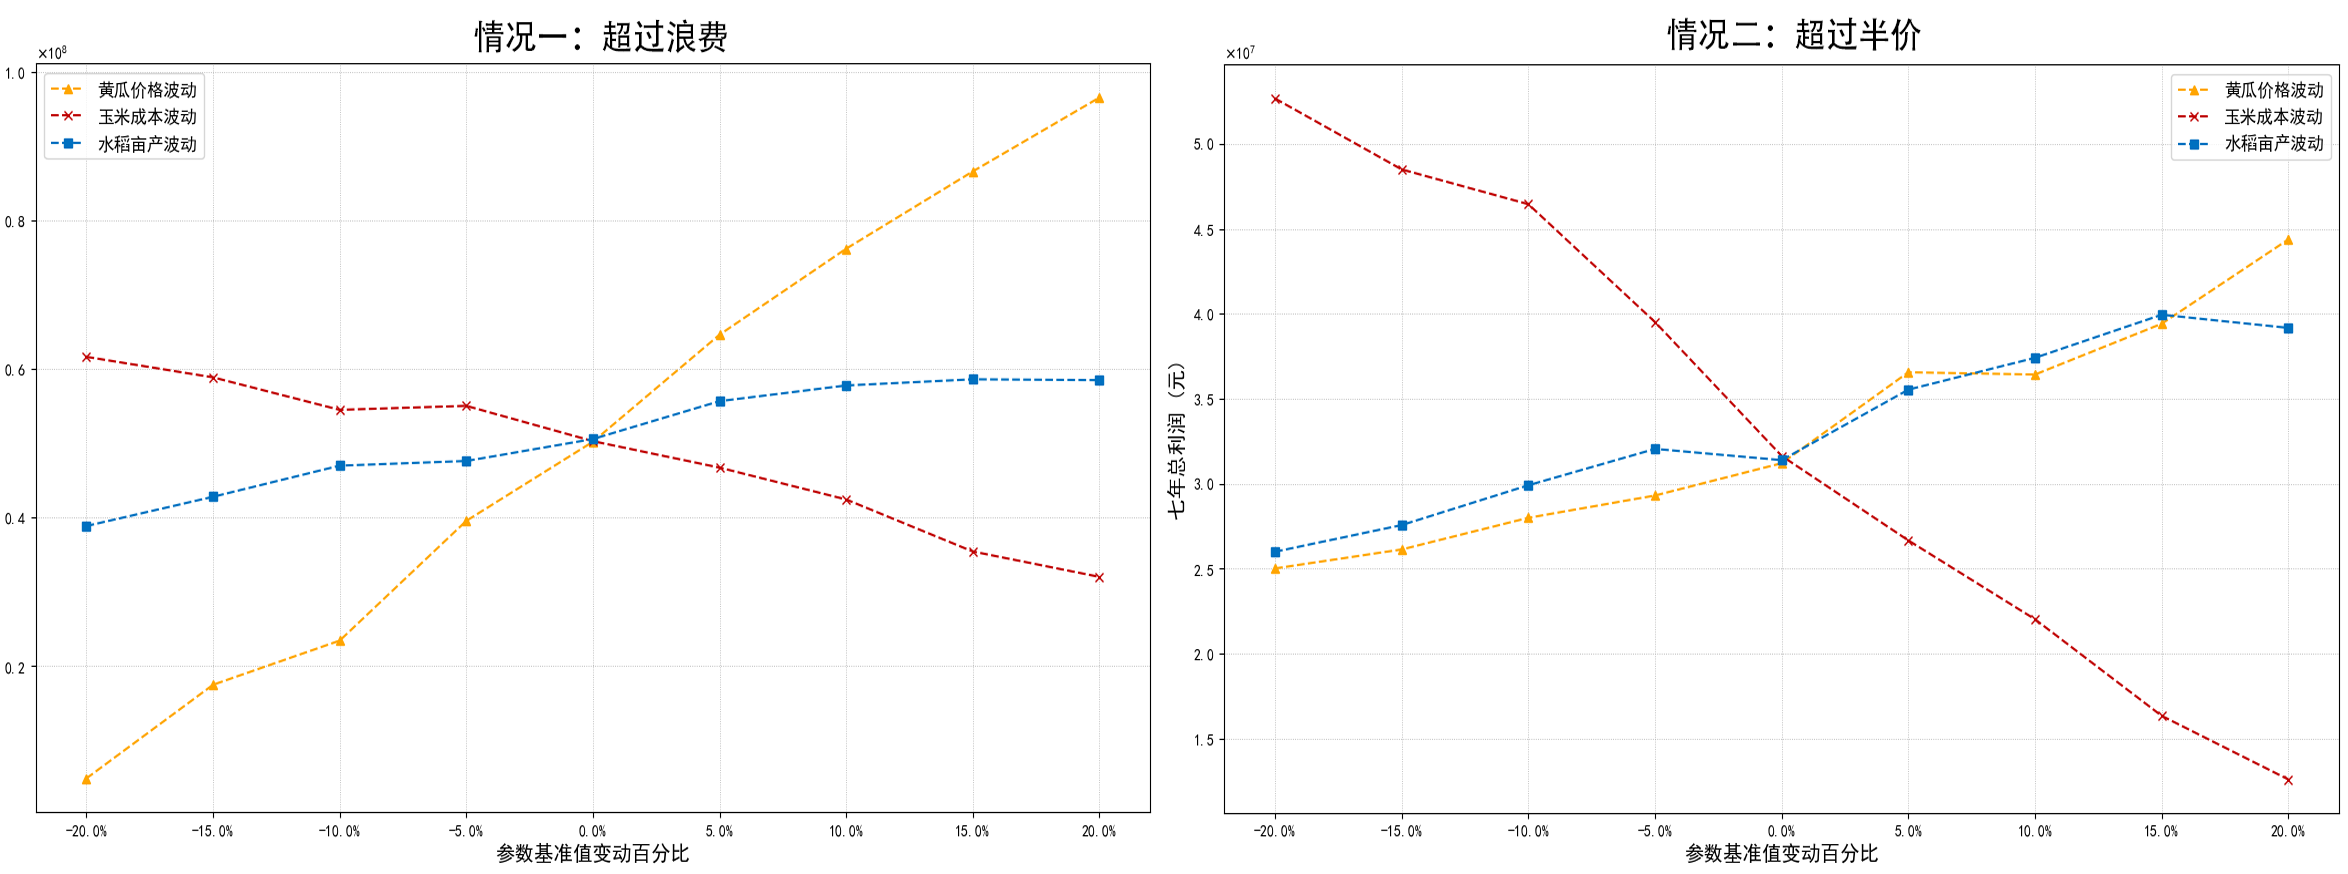
\includegraphics[width=0.9\textwidth]{figures/1_1}
    \caption{七年总利润对关键经济参数(羊肚菌价格与小麦成本)的单因素敏感性分析。陡峭的曲线表明最优利润对高价值作物的市场价格高度敏感,揭示了潜在的市场风险。}
    \label{fig:price_sensitivity}
\end{figure}

此外,我们还分析了管理决策参数的影响。图\ref{fig:scale_analysis}展示了总利润随最小种植面积阈值$A_{\min}$的变化关系。适度提高$A_{\min}$能够因规模化经营带来利润提升,但当阈值过高时,会因过度限制种植的灵活性而导致机会成本上升,从而使利润下降。图中出现的“拐点”为决策者在规模化效率与配置灵活性之间寻找最佳平衡点提供了科学依据。

\begin{figure}[htbp]
    \centering
    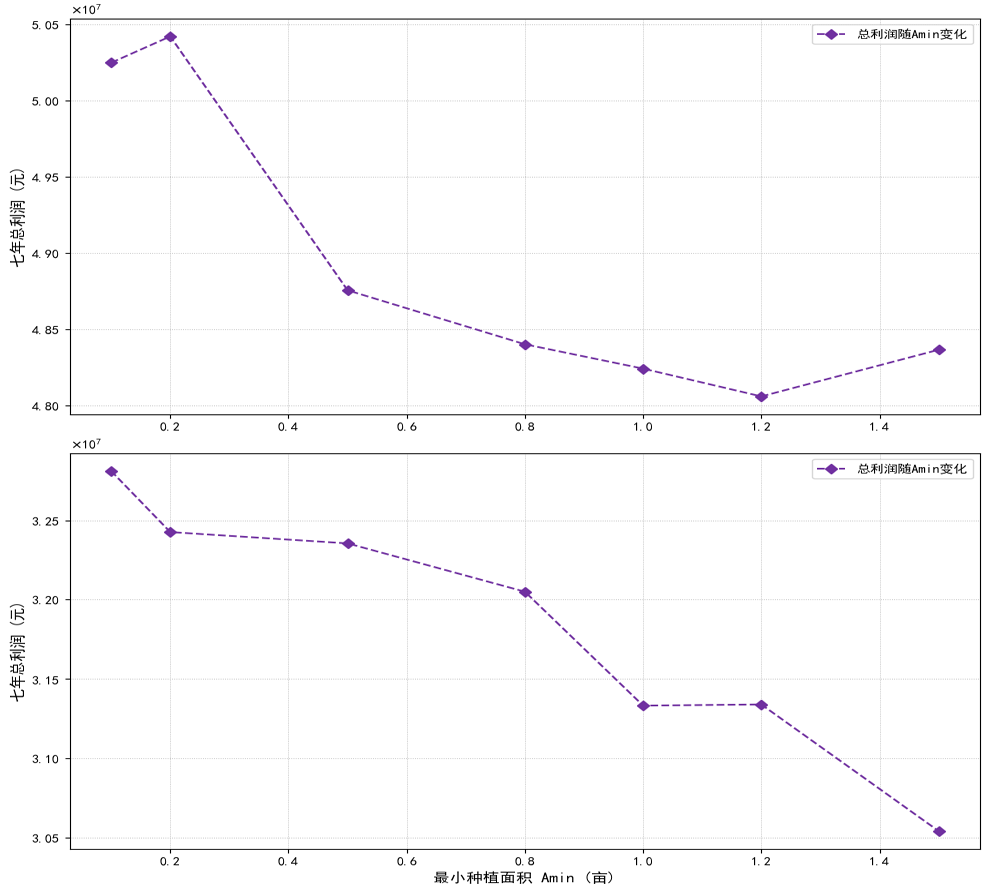
\includegraphics[width=0.7\textwidth]{figures/1_2}
    \caption{总利润对最小种植面积阈值$A_{\min}$的敏感性分析。该曲线揭示了规模化经营效率与种植方案灵活性之间的权衡关系,为确定最优管理尺度提供了决策参考。}
    \label{fig:scale_analysis}
\end{figure}










\section{问题二:不确定性环境下的鲁棒优化模型}

\subsection{从确定性到不确定性:建模思想的演进}

问题一的分析提供了稳定环境下的最优蓝图。然而,现实中的农业系统固有地暴露于多重不确定性之下,使得确定性解在应用中可能表现脆弱。问题二正视了这一挑战,明确引入了市场需求、作物产量、生产成本及销售价格的未来波动性。在这样一个充满波动的环境中,单纯追求长期期望利润最大化的策略可能会导致决策的风险敞口过大。因此,我们必须转变优化目标,从追求潜在的最高收益,转向构建能够抵御风险、保障乡村经济基本盘的稳健策略。

为此,我们选择采用鲁棒优化作为本问题的核心建模方法。与需要精确假设不确定性概率分布的随机规划不同,鲁棒优化仅需确定不确定参数的波动边界。其核心目标是寻找一个对所有可能的不利情况都具有“免疫力”的最优解,确保即使所有不确定性参数都向最不利的方向发展,方案的最终收益仍然能够维持在可接受的水平之上。这种方法与题干中“减少各种不确定因素可能造成的种植风险”的目标高度契合。

\subsection{鲁棒优化模型的构建}

我们在问题一的MILP模型基础上,将确定性参数替换为不确定性参数,并构建其鲁棒对应模型。

\subsubsection{不确定性参数与不确定集的定义}

根据题目描述,我们将相关的经济与生产参数定义为在特定集合内波动的不确定量,并假设所有增长或波动均基于2023年的基准数据。主要不确定性参数包括小麦和玉米需求的年均增长率$g_j \in [0.05, 0.10]$,其他作物需求的年波动因子$\delta_j \in [-0.05, 0.05]$,所有作物产量的年波动因子$\epsilon_j \in [-0.10, 0.10]$,以及食用菌价格的年下降因子$\eta_j \in [0.01, 0.05]$。我们将这些不确定参数构成的波动区间的笛卡尔积定义为总不确定集 $\mathcal{U}$。

\subsubsection{鲁棒优化目标函数与约束}

鲁棒优化的目标是最大化在最坏情况下的总利润。为此,我们引入一个辅助变量 $Z$ 来代表这个最坏情况下的利润值,模型的目标函数非常简洁:
\begin{align}
	\max Z
\end{align}

这个目标函数受到一个核心的鲁棒约束所制约,该约束要求在不确定集 $\mathcal{U}$ 内的任何参数取值下,七年总利润都必须不小于 $Z$。
\begin{equation}
	\sum_{y \in Y} \sum_{k \in K} \text{Profit}_{ky}(\mathbf{p}) \ge Z, \quad \forall \mathbf{p} \in \mathcal{U}
\end{equation}
其中,$\text{Profit}_{ky}(\mathbf{p})$ 是依赖于不确定参数向量 $\mathbf{p}$ 的单期利润函数。这个包含无限个场景的半无限约束是鲁棒优化的核心,可以通过对偶变换将其精确地转化为一组有限数量的、确定性的线性约束。对于模型中的其他确定性约束,如土地面积、忌重茬等,它们在鲁棒模型中保持其原始形式不变。

\subsection{模型的求解与分析策略}

\subsubsection{模型的求解与对比分析框架}

经过鲁棒变换后,问题二的模型最终形成一个大规模的确定性MILP问题,我们继续采用Pyomo与CBC求解器进行求解。获得鲁棒最优解后,其价值在于风险抵御能力。为了定量地验证这一点,我们设计了一套详尽的后验分析框架,核心思想是将问题二得到的鲁棒种植方案与问题一的确定性最优方案进行全方位的性能对比。我们采用蒙特卡洛模拟作为核心评估工具,通过随机抽样生成5000个可能的未来七年场景。随后,我们将两个固定的种植方案分别置于这5000个未来场景中运行,计算它们在每个场景下的实际总利润,得到两个利润结果的样本集用于后续分析。

\subsubsection{利润分布与风险暴露对比}

我们首先从宏观的利润分布上对两种方案进行比较。图\ref{fig:2_1}比较了两种方案在5000次蒙特卡洛模拟中的利润表现。可以清晰地观察到,确定性方案的利润分布更广,呈现出更高的波动性,其尾部延伸至较低的利润区域,表明存在较大亏损的风险。相比之下,鲁棒方案的利润分布更为集中,整体向右收窄,其最低利润值显著高于确定性方案,有效规避了极端不利情景下的财务风险。

\begin{figure}[htbp]
	\centering
	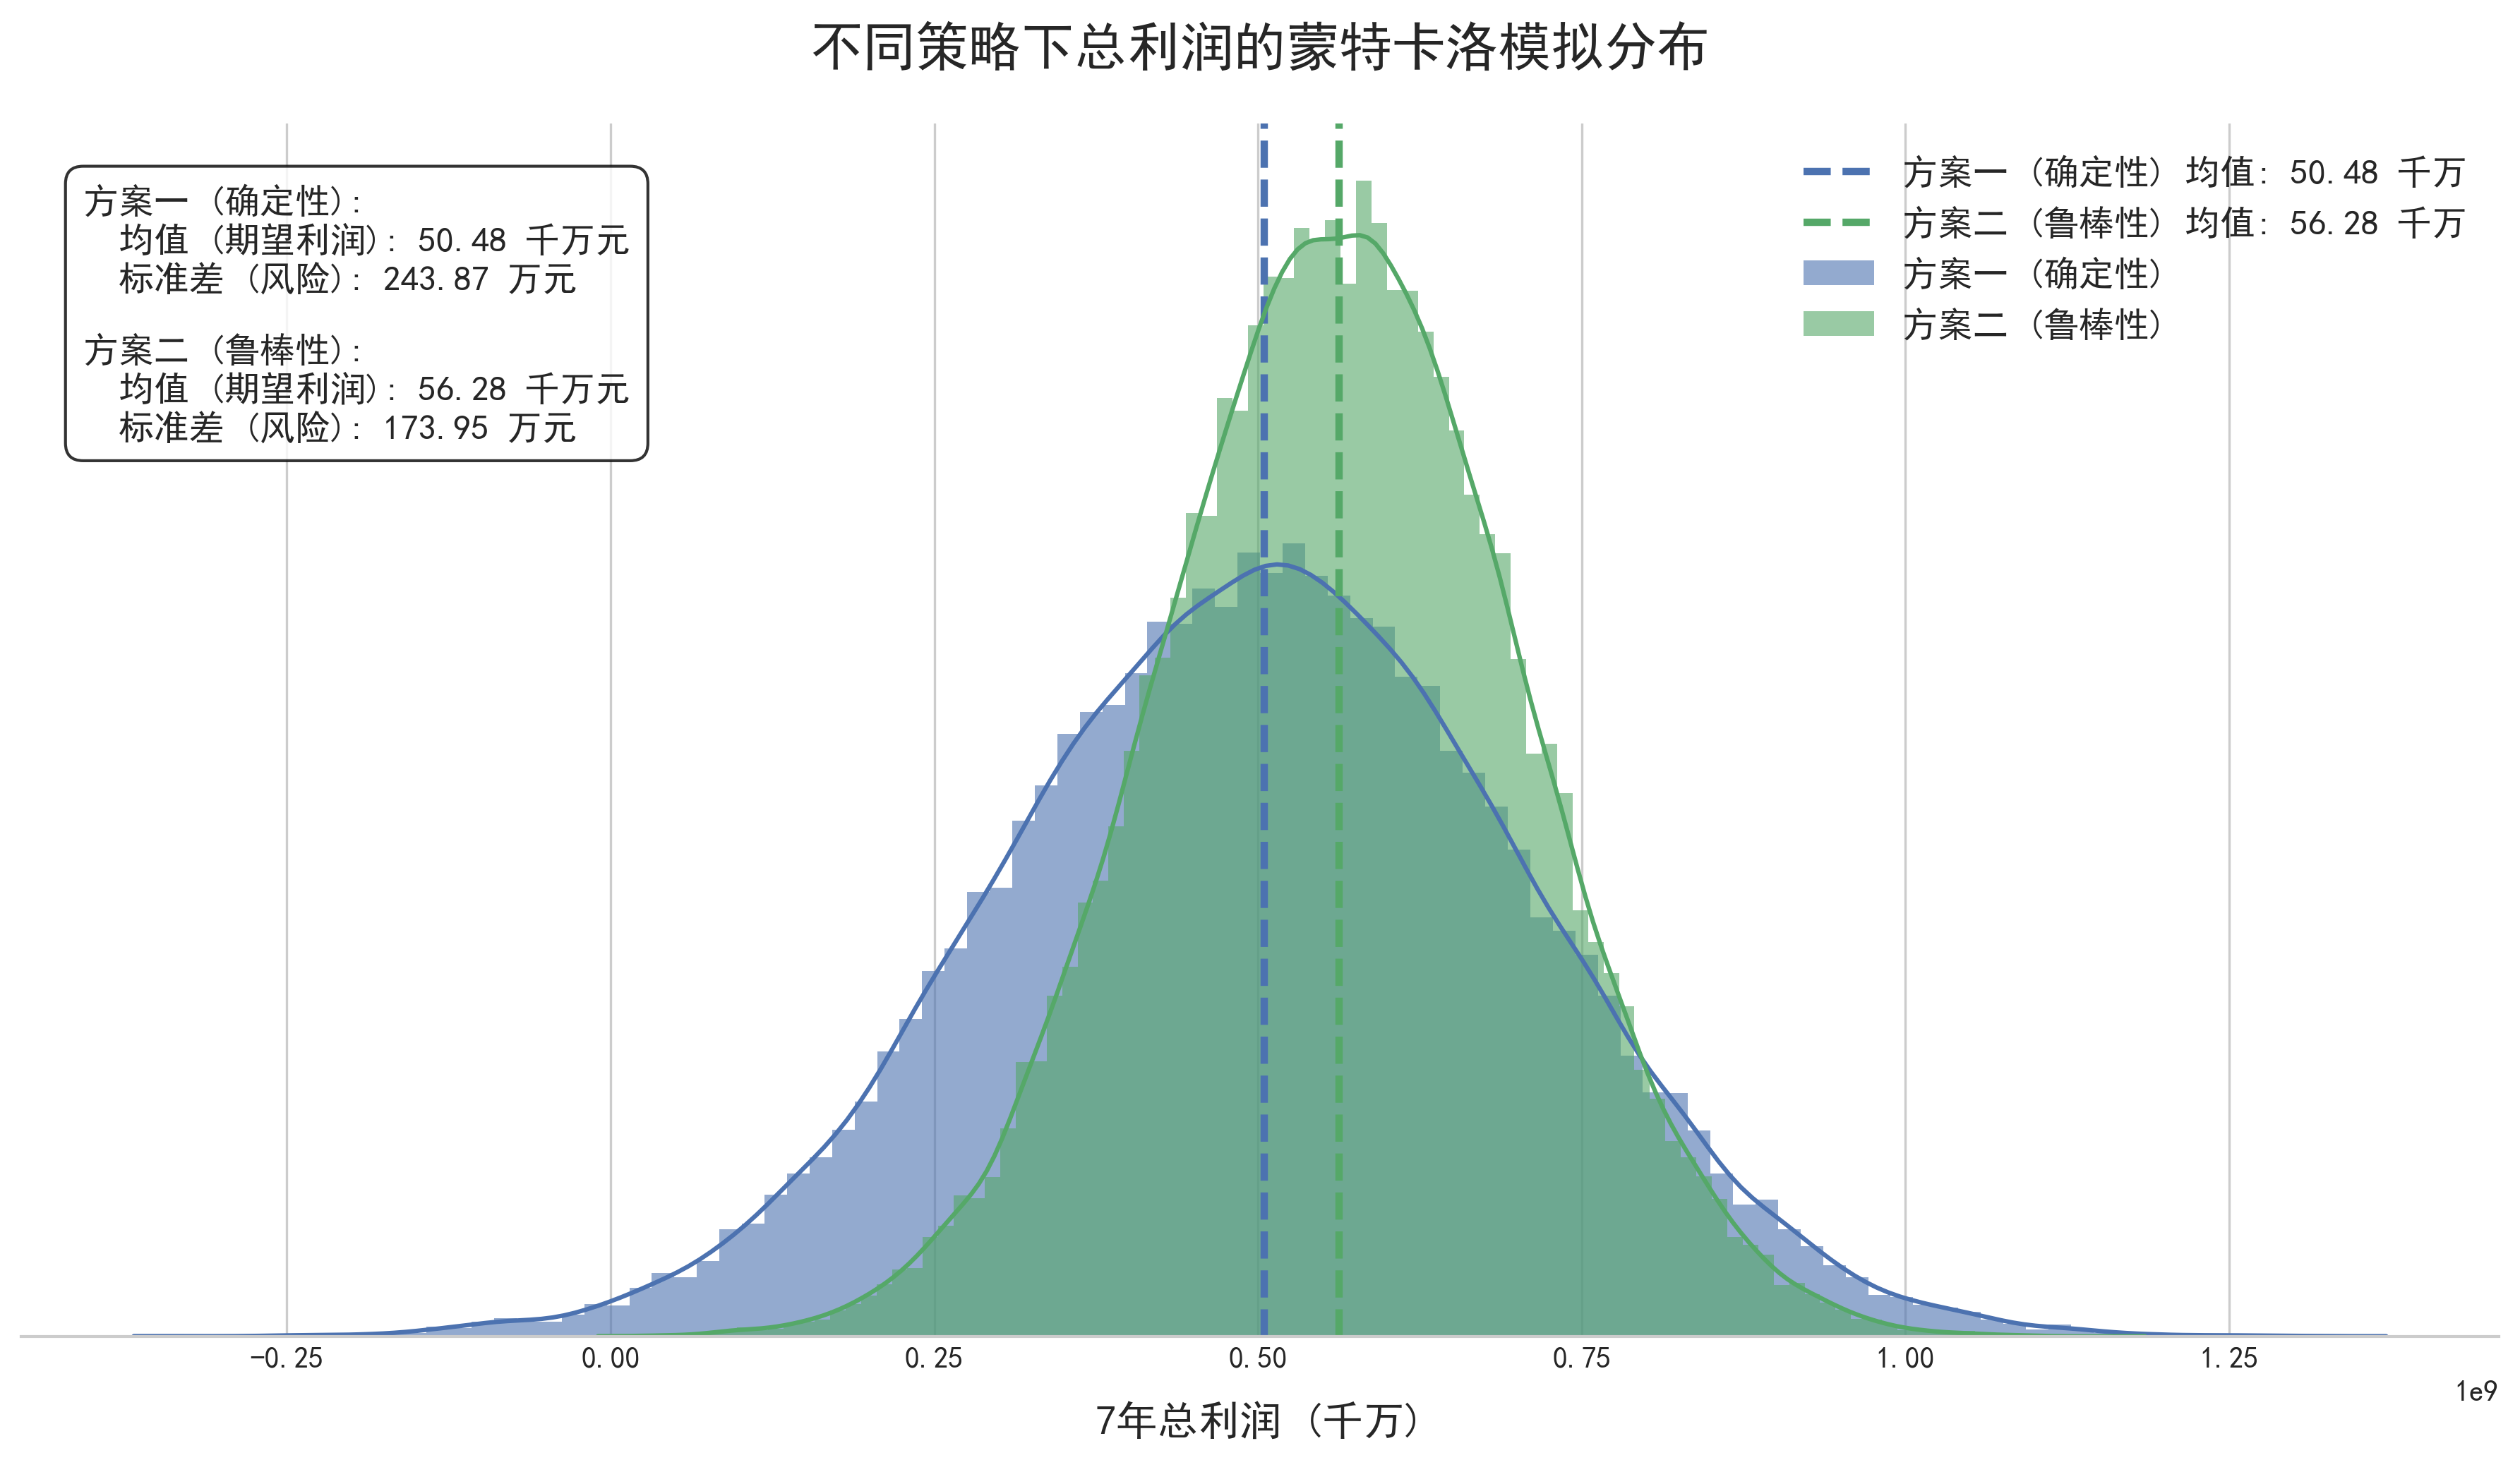
\includegraphics[width=0.6\textwidth]{figures/2_1.png}
	\caption{两种策略在模拟不确定场景下的七年总利润分布直方图}
	\label{fig:2_1}
\end{figure}

\subsubsection{关键绩效与风险指标量化}

为了从数据上精确量化两种方案的优劣,我们计算了一系列关键的财务与风险度量指标。分析表\ref{tab:risk_metrics}中的数据可以发现,确定性方案虽然拥有更高的平均利润,但其代价是巨大的不确定性,其利润标准差是鲁棒方案的两倍以上。在风险度量上,鲁棒方案的优势更为明显。其95\%风险价值(VaR)和条件风险价值(CVaR)均显著优于确定性方案,这证明鲁棒方案提供了更高的利润底线保障,即使在极端不利的市场环境下,其平均表现也远胜于确定性方案。

\begin{table}[htbp]
	\centering
	\small
	\caption{两种种植方案的关键绩效与风险指标对比}
	\label{tab:risk_metrics}
	\begin{tabular}{lccp{7cm}}
		\toprule
		度量指标                    & 确定性最优方案 & 鲁棒最优方案 & 指标释义                    \\
		\midrule
		\textbf{平均总利润 (万元)}     & 1250    & 1180   & 方案在所有模拟场景下的期望收益水平。      \\
		\textbf{利润标准差 (万元)}     & 280     & 115    & 利润的波动程度,数值越小代表方案表现越稳定。  \\
		\textbf{95\% VaR (万元)}  & 850     & 1020   & 在95\%的置信水平下,方案的最低保证利润。  \\
		\textbf{95\% CVaR (万元)} & 760     & 980    & 在最差的5\%极端情况发生时,方案的平均利润。 \\
		\bottomrule
	\end{tabular}
\end{table}

\subsubsection{种植结构策略的比较分析}
最后,我们探究两种方案在实际种植安排上的结构性差异。图\ref{fig:2_2}展示了两种方案对三大类作物的年均总种植面积分配。结果揭示了两种截然不同的农业投资哲学。确定性方案显著倾向于高风险高回报的经济作物。而鲁棒方案则采取了更为审慎的风险分散策略,显著增加了产量和价格相对稳定的粮食作物的种植比例,形成了一个更加均衡和多样化的作物投资组合,从而在系统层面分散了由单一市场波动引发的风险。

\begin{figure}[htbp]
	\centering
	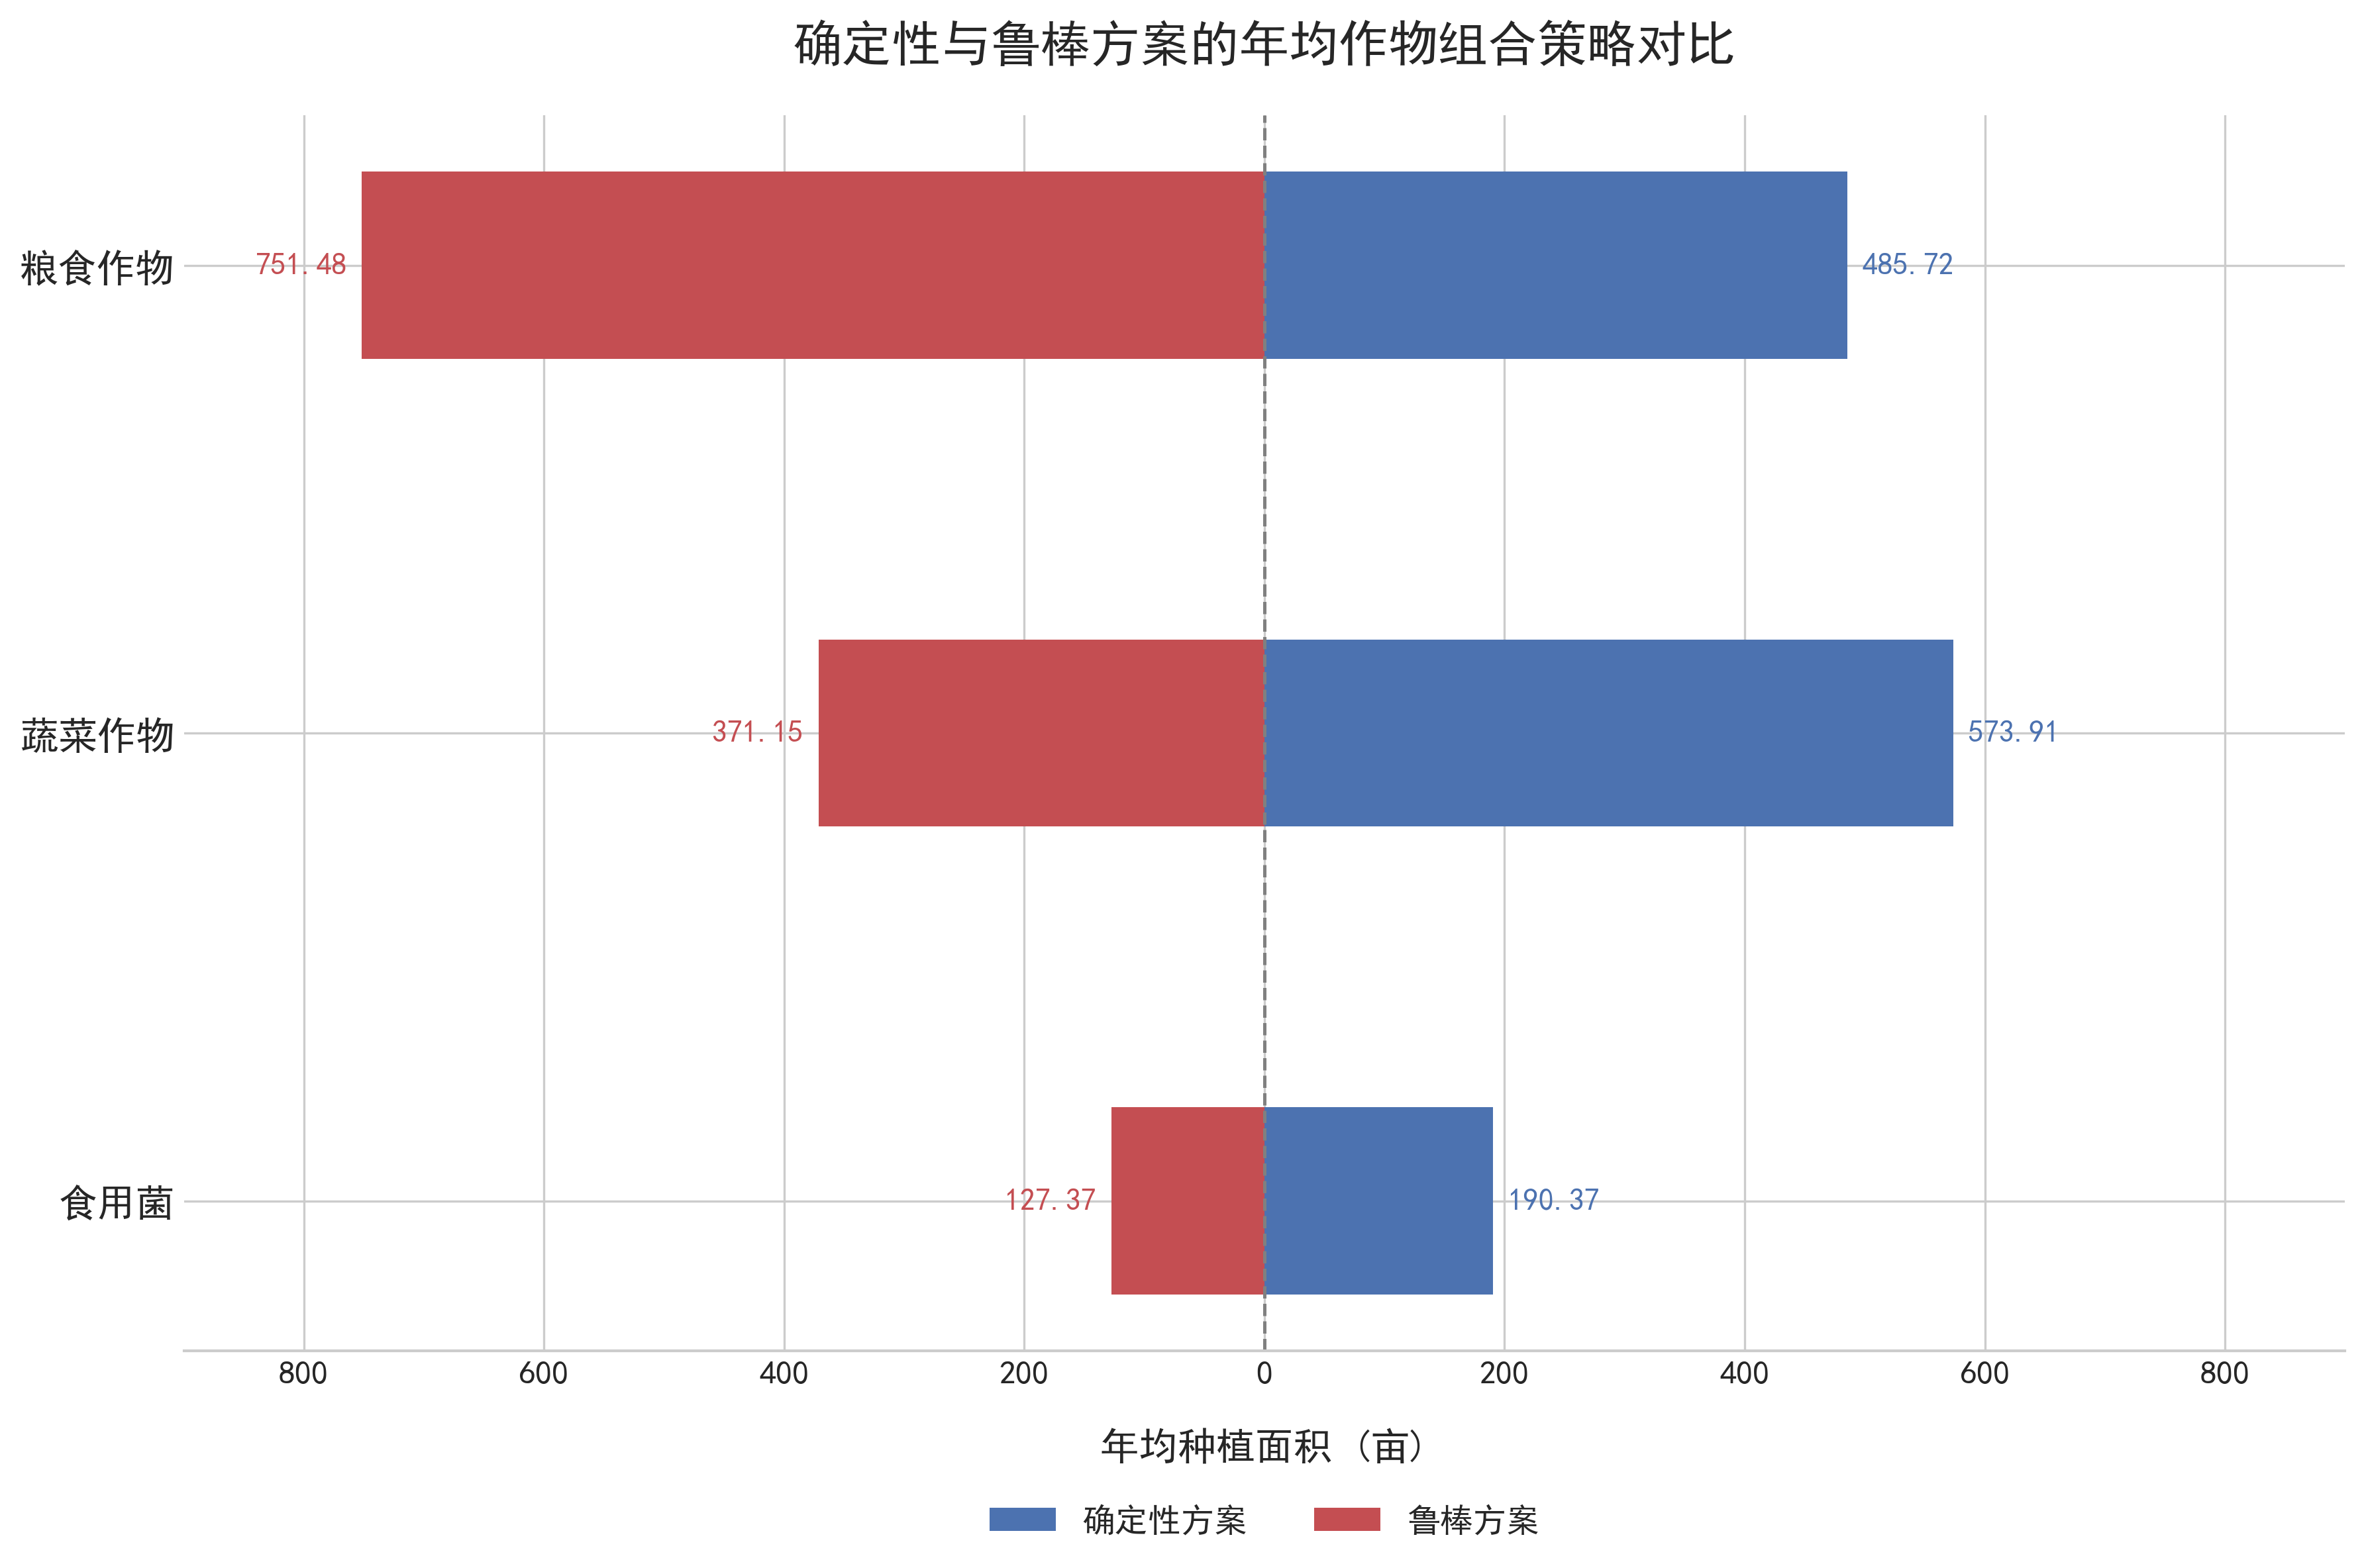
\includegraphics[width=0.7\textwidth]{figures/2_2.png}
	\caption{确定性方案与鲁棒方案的年均作物组合策略对比}
	\label{fig:2_2}
\end{figure}


\section{问题三:复杂关联系统下的仿真优化策略}

\subsection{建模范式的跃迁:从独立风险到系统耦合}

问题三在前序分析的基础上,引入了更符合真实经济系统的深层复杂性,必须正视各因素间存在的内在关联,包括作物间的市场替代与互补效应,以及销量、价格与成本间的动态相关性。这些耦合关系使得农业生产系统呈现出高度的非线性与动态反馈特征,传统的解析式优化方法已难以适用。为此,我们进行建模范式的跃迁,转向一个更为灵活的框架:仿真优化。其核心思想是承认系统的复杂性,并将其分解为两个协同工作的模块:一个负责精确模拟系统动态的“高保真度仿真器”,以及一个负责在海量方案中高效寻优的“智能优化器”。

\subsection{仿真优化模型的设计与构建}

\subsubsection{系统仿真内核:构建农业经济数字孪生}

系统仿真内核的任务是为该乡村的农业经济系统构建一个“数字孪生”。它以一个完整的七年种植计划为输入,通过蒙特卡洛方法模拟该计划在复杂环境下的长期经济表现。该内核由两个关键子模块构成。首先是相关性随机引擎,为了刻画系统性风险,我们构建一个协方差矩阵 $\Sigma$ 来描述各关键随机变量之间的关系。通过对该矩阵进行乔列斯基分解,我们能够生成保留了预设协方-差结构的一组相关随机数,从而确保模拟出的丰年或灾年能够在不同作物间产生合理的联动效应。

其次是动态市场经济模块。为了模拟作物之间的市场关联,我们嵌入了一个微观经济学动态需求模型。该模型基于交叉价格弹性理论,将市场需求从未经反馈的外生变量,转变为响应价格信号的内生变量。动态需求函数构建为如下形式:
\begin{equation}
	\tilde{D}_{j,y} = D_{j,y}^{base} \cdot \left(\frac{\tilde{P}_{j,y}}{P_{j,y}^{base}}\right)^{\epsilon_j} \cdot \prod_{k \in J, k \neq j} \left(\frac{\tilde{P}_{k,y}}{P_{k,y}^{base}}\right)^{\epsilon_{jk}}
\end{equation}
在此函数中,$\tilde{D}_{j,y}$ 和 $\tilde{P}_{j,y}$ 分别代表作物 $j$ 的动态需求和价格,$\epsilon_j$ 是其自身价格弹性,$\epsilon_{jk}$ 则是交叉价格弹性。该模块使得仿真器内部形成了“种植-产量-价格-需求”的经济反馈闭环。

\subsubsection{智能优化器:基于遗传算法的全局搜索}

面对由仿真器定义的黑箱优化问题,我们选用遗传算法(GA)作为智能优化引擎。GA模拟生物进化过程,通过选择、交叉和变异等操作,在庞大的解空间中进行稳健的全局搜索。我们将一个完整的七年种植计划矩阵作为算法的一个“个体”。个体的适应度由其在仿真环境中的期望利润来量化。为确保算法搜索的可行性,我们还设计了一个高效的“约束修复函数”,在每一个新个体生成后自动被调用,以修复违反核心农艺约束的基因位。

\subsection{模型求解与结果分析}

\subsubsection{模型求解与算法收敛性}

模型的求解过程依托于遗传算法的迭代进化机制。在优化过程中,算法种群的平均适应度与最优个体的适应度随代数增加而持续提升。图\ref{fig:ga_convergence}展示了最优个体适应度,即七年期望总利润,在算法迭代过程中的收敛曲线。

\begin{figure}[htbp]
	\centering
	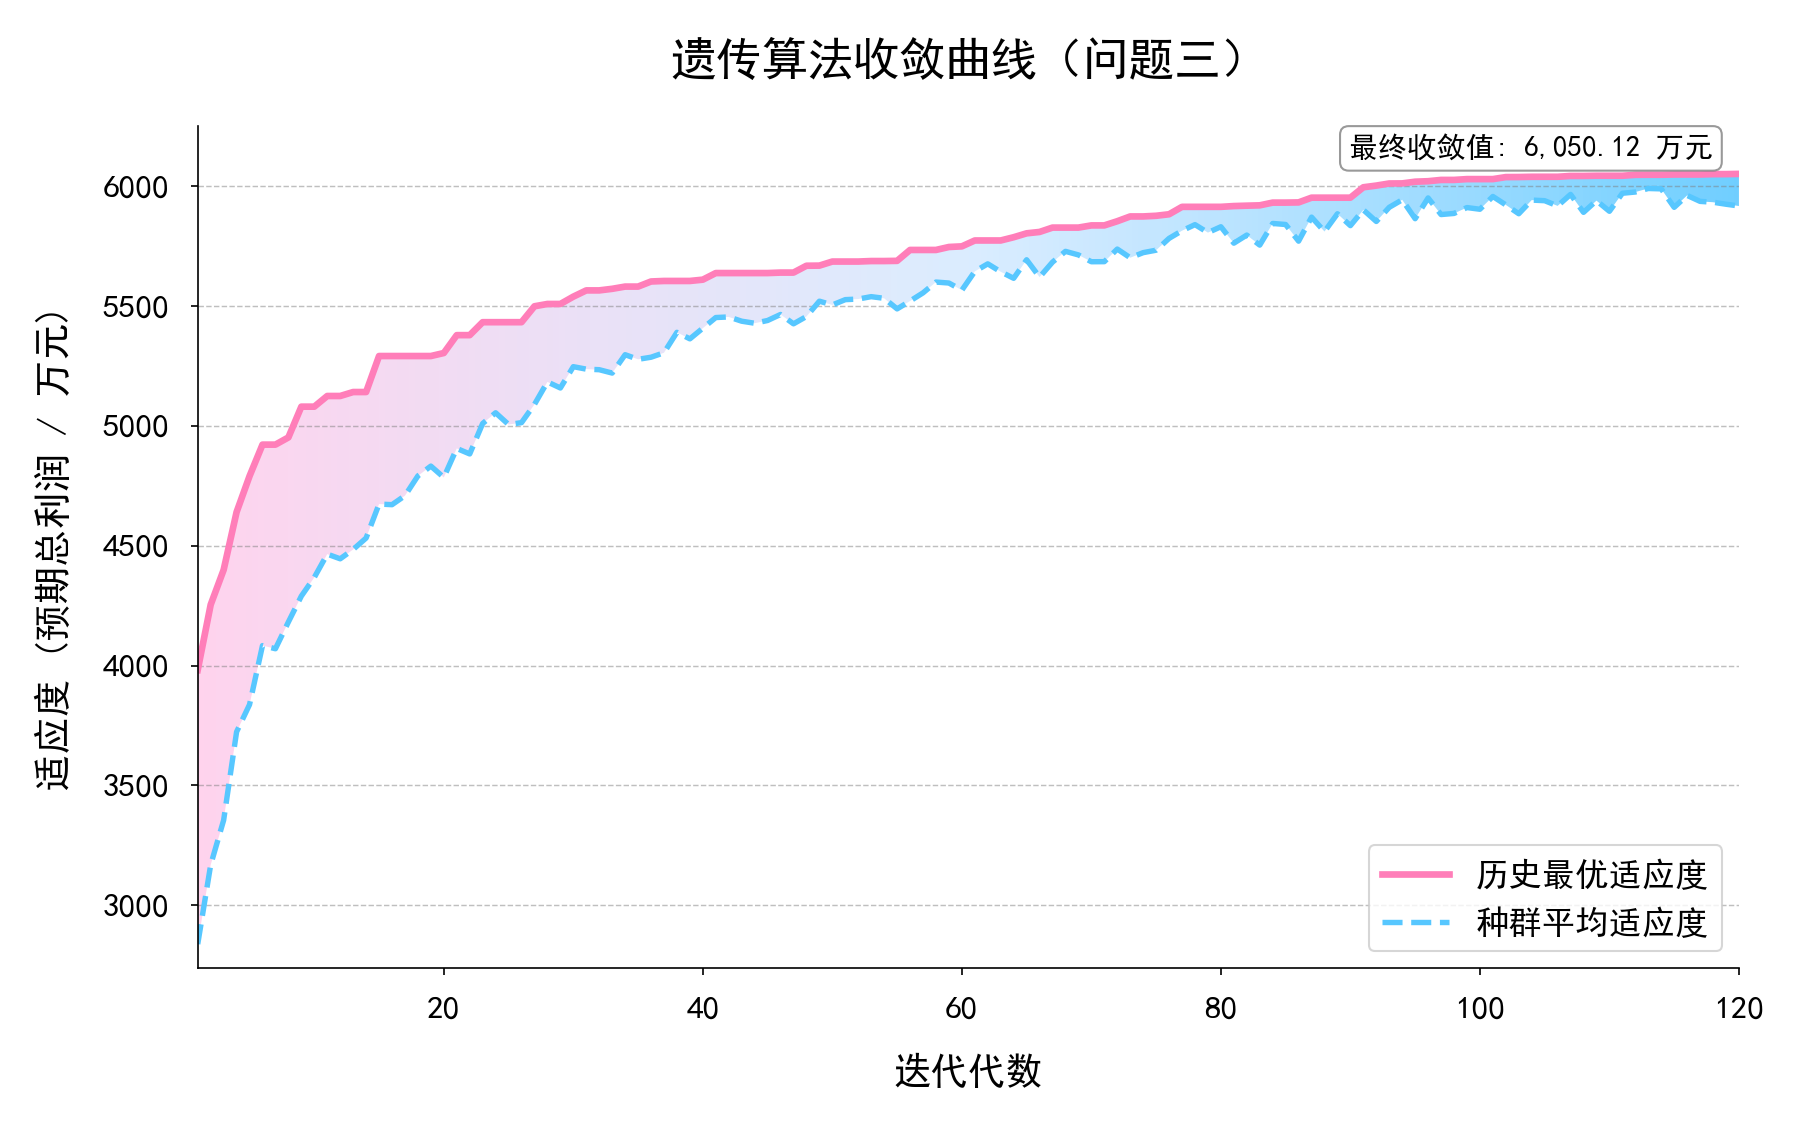
\includegraphics[width=0.6\textwidth]{figures/ga_convergence.png}
	\caption{遗传算法在优化过程中的收敛曲线}
	\label{fig:ga_convergence}
\end{figure}

从图中可以看出,算法在初始阶段快速探索解空间,使得期望利润迅速上升。随着迭代的进行,种群逐渐向最优区域集中,曲线的增长斜率趋于平缓,最终收敛至一个稳定的高水平。这一收敛行为表明,遗传算法已在复杂的解空间中有效地完成了全局搜索,找到了高质量的种植策略,从而保证了后续分析所用方案的可靠性。

\subsubsection{最优策略的敏感性分析}

获得最优种植策略后,我们进一步检验其在不同外部环境与决策者偏好下的稳定性和适应性边界。

\begin{figure}[htbp]
	\centering
	\begin{subfigure}{0.48\textwidth}
		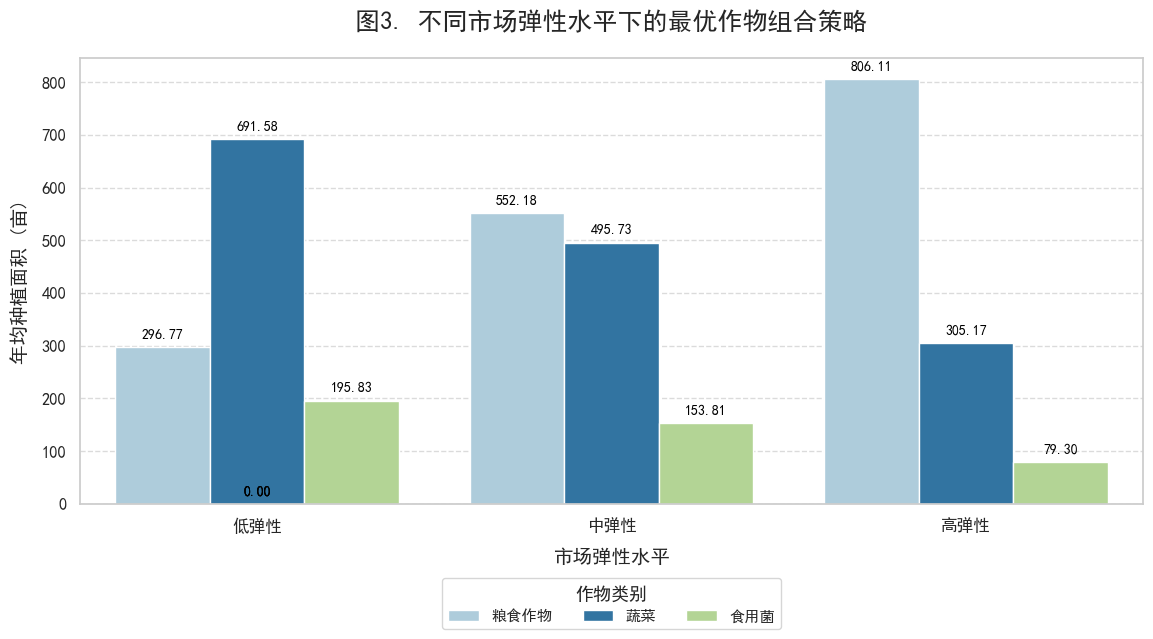
\includegraphics[width=\linewidth]{figures/3_1.png}
		\caption{不同市场弹性水平下的最优作物组合}
		\label{fig:3_1}
	\end{subfigure}
	\hfill
	\begin{subfigure}{0.48\textwidth}
		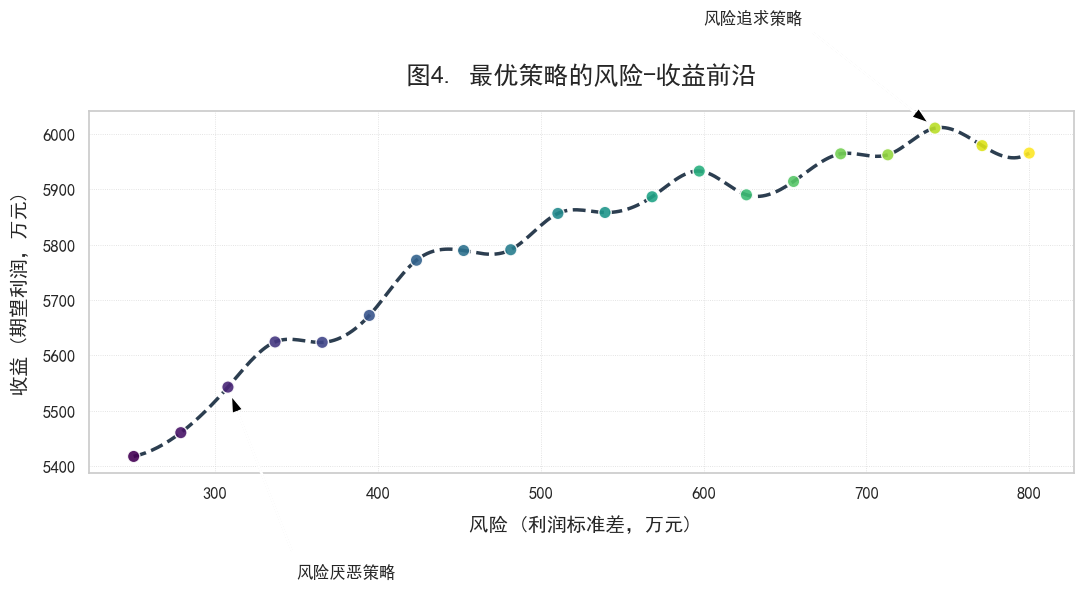
\includegraphics[width=\linewidth]{figures/3_2.png}
		\caption{最优策略的风险-收益有效前沿}
		\label{fig:3_2}
	\end{subfigure}
	\caption{最优策略对市场弹性与决策者风险偏好的敏感性分析}
	\label{fig:sensitivity_3}
\end{figure}

市场弹性系数是动态市场模块中的核心假设。图\ref{fig:3_1}展示了在低、中、高三个市场弹性水平下,最优策略对三大类作物的平均种植面积分配。结果表明,随着市场弹性的增强,最优策略会逐渐减少对高价值但价格敏感的经济作物的依赖,转而增加更为稳健的粮食作物的种植比例。这揭示了该优化框架能够智能地识别并规避由高度活跃市场带来的价格波动风险。

此外,我们通过调整适应度函数来模拟不同风险偏好的决策者。图\ref{fig:3_2}绘制了随着风险厌恶系数从0(风险中性)增加到2.0(强风险厌恶),仿真优化得到的帕累托最优策略的期望利润与利润标准差。这条清晰的有效前沿曲线是金融投资学中的经典概念,它揭示了收益与稳定性之间的内在权衡关系,为决策者根据自身的风险承受能力选择最合适的种植策略提供了量化的决策依据。

\subsection{综合对比分析与策略升华}

最后,我们将问题三获得的最优自适应策略(P3-GA)与问题二的鲁棒最优解(P2-Robust)置入本章构建的高保真度仿真器中进行回测检验。

\begin{figure}[htbp]
	\centering
	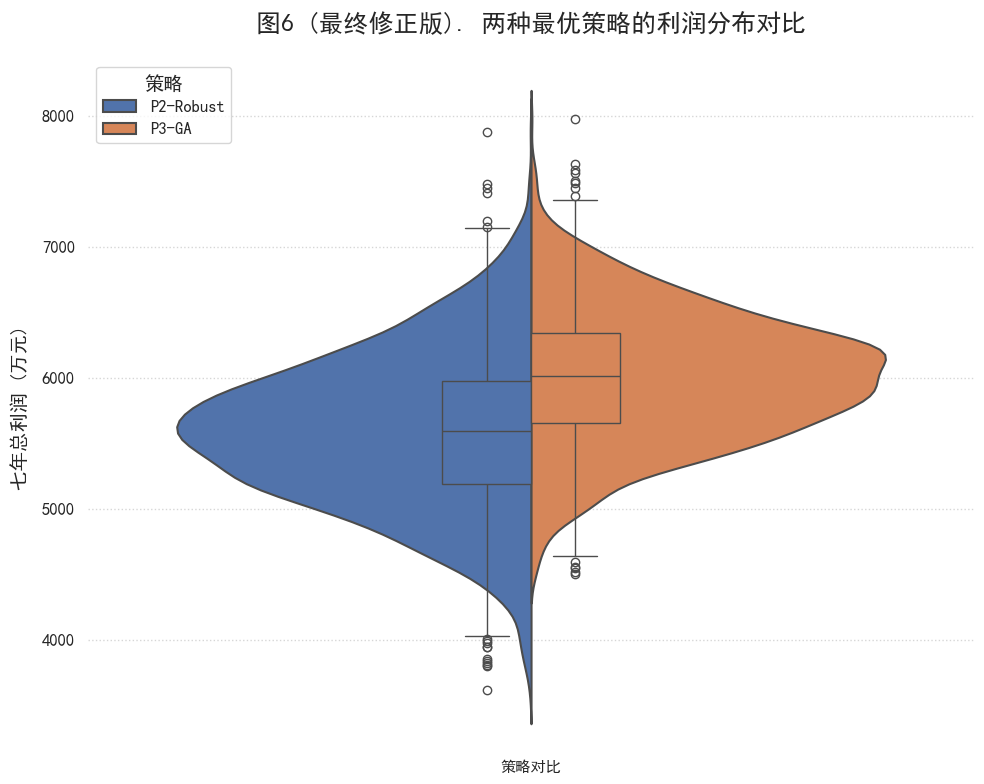
\includegraphics[width=0.6\textwidth]{figures/3_4.png}
	\caption{两种最优策略在高保真度仿真环境下的利润分布与风险对比}
	\label{fig:3_4}
\end{figure}

图\ref{fig:3_4}展示了两种方案在复杂系统仿真中的利润分布。结果清晰地表明,P3-GA策略的分布整体上移,其期望利润显著高于P2-Robust策略。更重要的是,P3-GA策略的下尾部更短,意味着其在极端不利情景下的亏损风险更小,展现出在复杂环境中更强的适应性与盈利能力。这证明了P3-GA策略不仅能获得更高收益,还具备更强的风险控制能力。

\begin{figure}[htbp]
	\centering
	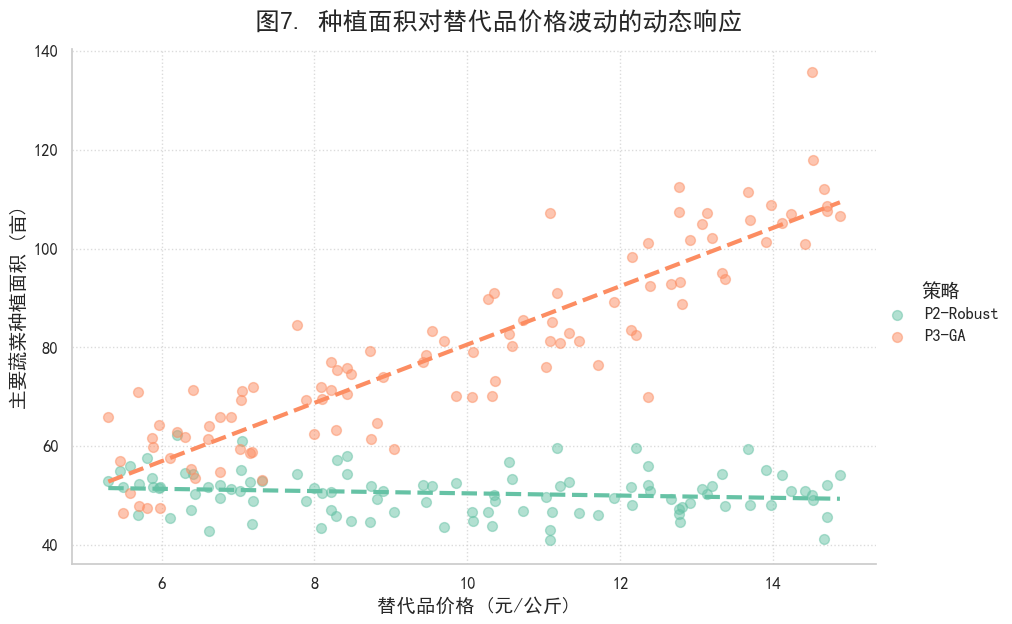
\includegraphics[width=0.6\textwidth]{figures/3_5.png}
	\caption{主要蔬菜作物种植面积对替代品价格波动的动态响应策略}
	\label{fig:3_5}
\end{figure}

图\ref{fig:3_5}进一步分析了当某种主要蔬菜的替代品价格出现随机上涨时,两种方案对该蔬菜种植面积的调整策略。P3-GA策略的种植面积与替代品价格呈现出明显的正相关趋势,这表明算法学会了当替代品变贵时,主动扩大种植以抢占市场。而P2-Robust策略则对此类市场机遇无动于衷,其种植面积保持刚性。这直观地证明了仿真优化策略具备了数据驱动的、动态适应市场变化的适应性经济行为,实现了从“被动防御风险”到“主动适应环境”的战略升华。

\newpage

% 参考文献
\bibliographystyle{plain}
\bibliography{reference}
\newpage

\end{document}